\documentclass[12pt,a4paper]{article}

% Packages
\usepackage[utf8]{inputenc}
\usepackage[english]{babel}
\usepackage{amsmath,amssymb,amsthm}
\usepackage{graphicx}
\usepackage{geometry}
\usepackage{float}
\usepackage{caption}
\usepackage{subcaption}
\usepackage{hyperref}
\usepackage{siunitx}
\usepackage{booktabs}
\usepackage{bm}
\usepackage{pdfpages}
\usepackage{tikz}

% Page geometry
\geometry{margin=2.5cm}

% Custom commands
\newcommand{\parder}[2]{\frac{\partial #1}{\partial #2}}
\newcommand{\pparder}[2]{\frac{\partial^2 #1}{\partial {#2}^2}}
\newcommand{\Rey}{\text{Re}}
\newcommand{\Pran}{\text{Pr}}

\begin{document}

% Title page
\begin{titlepage}
    \centering
    \vspace*{2cm}

    {\Huge\bfseries Development of Flow at the Entrance of a Cylindrical Pipe\par}

    \vspace{1.5cm}

    {\Large Numerical Simulation and Modelling of Incompressible Flow\par}

    \vspace{1cm}

    {\large LV-Nr.: 321.053 EX\par}
    {\large Winter Semester 2025/26\par}

    \vfill

    {\Large
    Felix Scope\\
    \texttt{felix\_scope@yahoo.de}\\
    }

    \vfill

    {\large \today\par}
\end{titlepage}

\tableofcontents
\newpage

% Include the assignment (as per guidelines)
\section*{Assignment}
\addcontentsline{toc}{section}{Assignment}
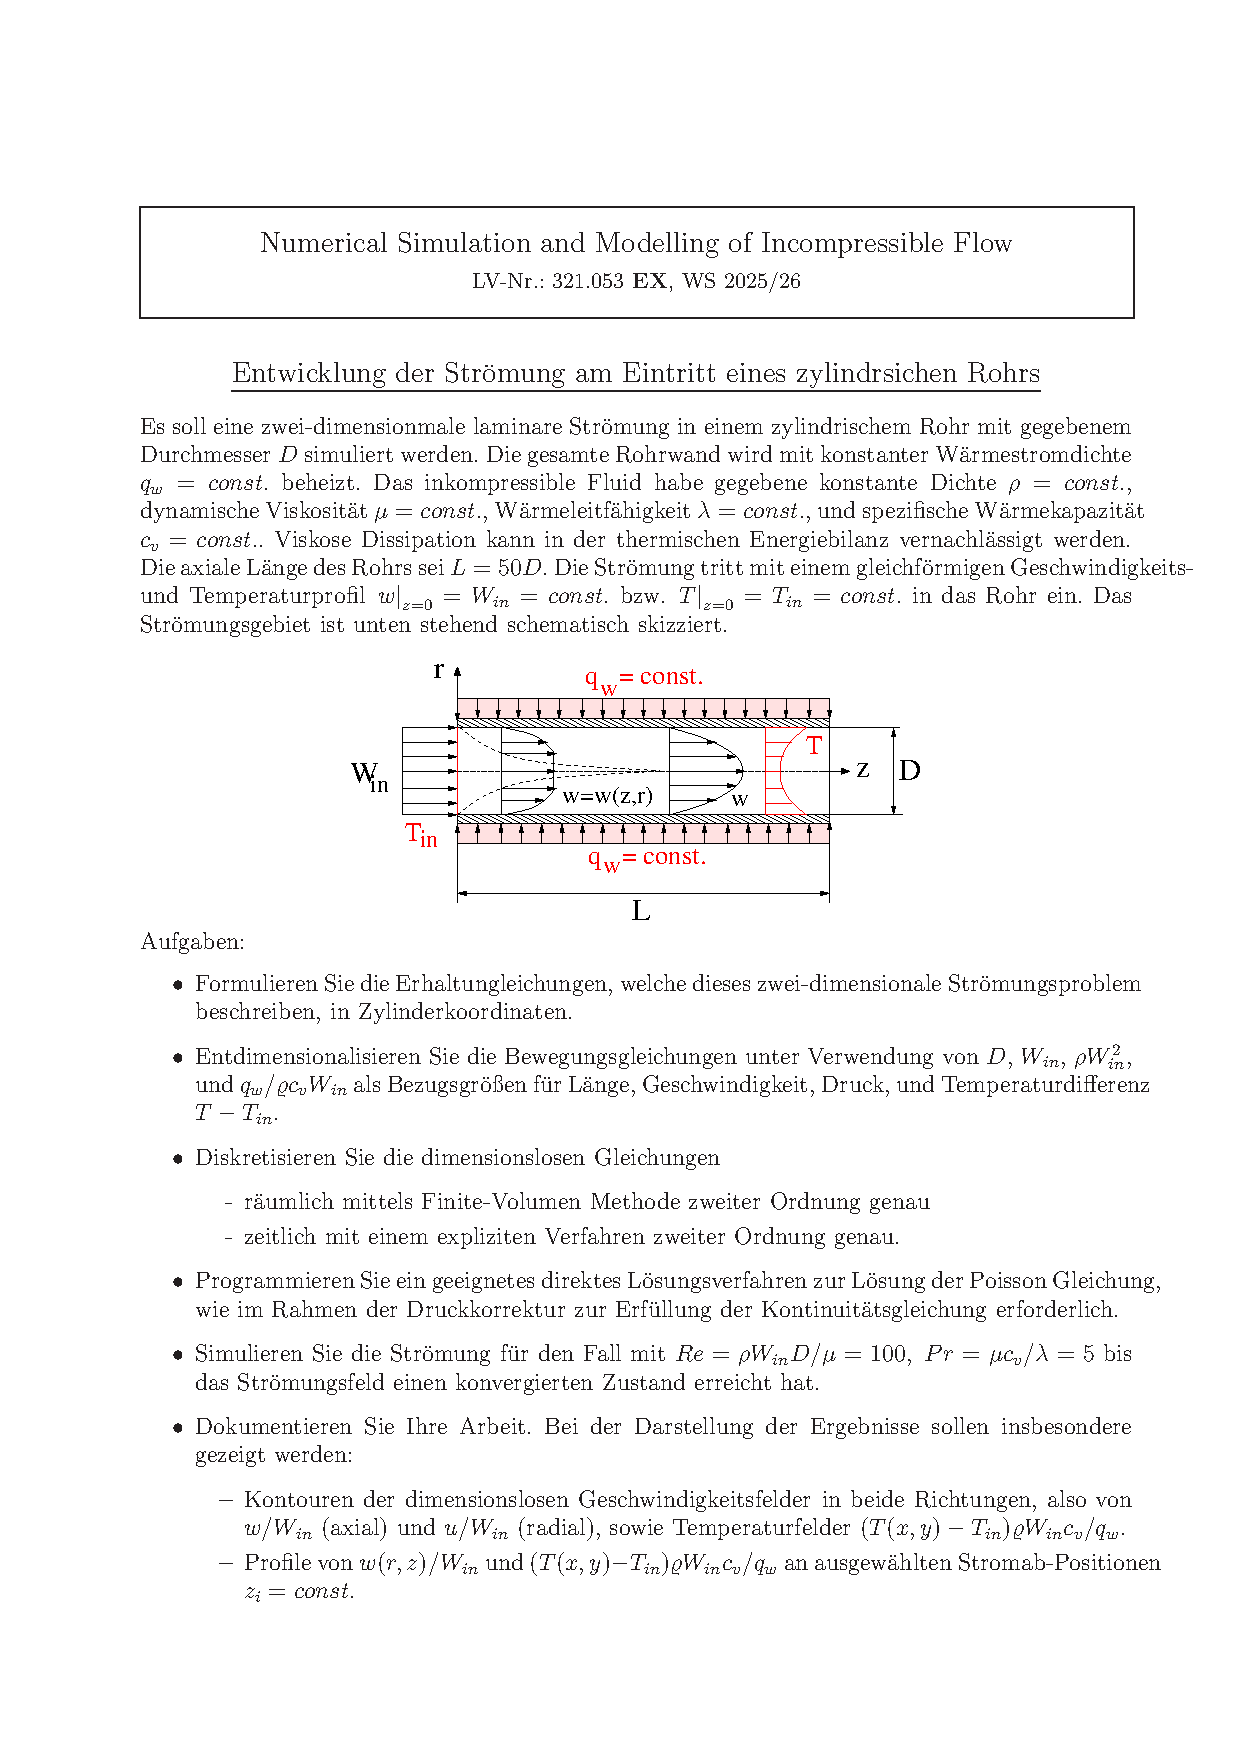
\includepdf[pages=-]{../Assignemnt/Assignment_WS25.pdf}

\newpage

\section{Problem Description}

\subsection{Geometry and Setup}

The problem considers a two-dimensional laminar flow in a cylindrical pipe with diameter $D$ and length $L = 50D$. The entire pipe wall is heated with constant heat flux $q_w = \text{const.}$ The incompressible fluid has constant properties: density $\rho$, dynamic viscosity $\mu$, thermal conductivity $\lambda$, and specific heat capacity $c_v$. Viscous dissipation is neglected in the thermal energy balance.

The flow enters the pipe with uniform velocity and temperature profiles:
\begin{align}
    w\big|_{z=0} &= W_{\text{in}} = \text{const.} \\
    T\big|_{z=0} &= T_{\text{in}} = \text{const.}
\end{align}

The computational domain is shown schematically in Figure~\ref{fig:geometry}.

\begin{figure}[H]
    \centering
    
\includegraphics[width=0.95\textwidth]{../Plots_python/geometry_diagram.png}
    \caption{Schematic of the cylindrical pipe flow with constant wall heat flux. Flow enters with uniform velocity $W_{\text{in}}$ and temperature $T_{\text{in}}$, and develops into a parabolic profile along the pipe length.}
    \label{fig:geometry}
\end{figure}

\subsection{Physical Parameters}

\begin{itemize}
    \item Reynolds number: $\Rey = \frac{\rho W_{\text{in}} D}{\mu} = 100$
    \item Prandtl number: $\Pran = \frac{\mu c_v}{\lambda} = 5$
    \item Length-to-diameter ratio: $L/D = 50$
\end{itemize}

\newpage

\section{Mathematical Formulation}

\subsection{Governing Equations in Cylindrical Coordinates}

For an axisymmetric flow in cylindrical coordinates $(r, z)$ with velocity components $(u, w)$ in the radial and axial directions respectively, the governing equations are:

\subsubsection{Continuity Equation}

The continuity equation for an incompressible fluid is:
\begin{equation}
    \parder{u}{r} + \frac{u}{r} + \parder{w}{z} = 0
    \label{eq:continuity_dim}
\end{equation}

\subsubsection{Momentum Equations}

The Navier-Stokes equations in cylindrical coordinates for axisymmetric flow are:

\textbf{Radial momentum:}
\begin{equation}
    \parder{u}{t} + u\parder{u}{r} + w\parder{u}{z} = -\frac{1}{\rho}\parder{p}{r} + \nu\left(\pparder{u}{r} + \frac{1}{r}\parder{u}{r} - \frac{u}{r^2} + \pparder{u}{z}\right)
    \label{eq:momentum_r_dim}
\end{equation}

\textbf{Axial momentum:}
\begin{equation}
    \parder{w}{t} + u\parder{w}{r} + w\parder{w}{z} = -\frac{1}{\rho}\parder{p}{z} + \nu\left(\pparder{w}{r} + \frac{1}{r}\parder{w}{r} + \pparder{w}{z}\right)
    \label{eq:momentum_z_dim}
\end{equation}

where $\nu = \mu/\rho$ is the kinematic viscosity.

\subsubsection{Energy Equation}

The energy equation (neglecting viscous dissipation) is:
\begin{equation}
    \parder{T}{t} + u\parder{T}{r} + w\parder{T}{z} = \alpha\left(\pparder{T}{r} + \frac{1}{r}\parder{T}{r} + \pparder{T}{z}\right)
    \label{eq:energy_dim}
\end{equation}

where $\alpha = \lambda/(\rho c_v)$ is the thermal diffusivity.

\subsection{Boundary Conditions}

\textbf{Inlet} ($z = 0$):
\begin{align}
    u(r, 0) &= 0 \\
    w(r, 0) &= W_{\text{in}} \\
    T(r, 0) &= T_{\text{in}}
\end{align}

\textbf{Wall} ($r = D/2$):
\begin{align}
    u(D/2, z) &= 0 \\
    w(D/2, z) &= 0 \\
    \lambda\parder{T}{r}\bigg|_{r=D/2} &= q_w
\end{align}
(Heat flows into the fluid at the wall, so with $r$ increasing outward this is a
positive gradient: the wall is hotter than the centerline.)

\textbf{Centerline} ($r = 0$, symmetry):
\begin{align}
    u(0, z) &= 0 \\
    \parder{w}{r}\bigg|_{r=0} &= 0 \\
    \parder{T}{r}\bigg|_{r=0} &= 0
\end{align}
($u=0$ is the essential (Dirichlet) condition here for the antisymmetric radial
velocity -- not interchangeable with $\partial u/\partial r=0$, which is a symmetry
statement appropriate for the even quantities $w$, $T$, not the primary condition on $u$.)

\textbf{Outlet} ($z = L$):
\begin{equation}
    \parder{u}{z}\bigg|_{z=L} = 0, \quad \parder{w}{z}\bigg|_{z=L} = 0, \quad \parder{T}{z}\bigg|_{z=L} = 0
\end{equation}

\newpage

\section{Non-Dimensionalization}

\subsection{Reference Scales}

We introduce the following reference scales:
\begin{itemize}
    \item Length: $D$
    \item Velocity: $W_{\text{in}}$
    \item Pressure: $\rho W_{\text{in}}^2$
    \item Temperature difference: $\frac{q_w}{\rho c_v W_{\text{in}}}$
\end{itemize}

\subsection{Non-Dimensional Variables}

Define the non-dimensional variables (denoted with asterisks):
\begin{align}
    r^* &= \frac{r}{D}, \quad z^* = \frac{z}{D} \\
    u^* &= \frac{u}{W_{\text{in}}}, \quad w^* = \frac{w}{W_{\text{in}}} \\
    p^* &= \frac{p}{\rho W_{\text{in}}^2} \\
    \theta &= \frac{(T - T_{\text{in}})\rho c_v W_{\text{in}}}{q_w} \\
    t^* &= \frac{t W_{\text{in}}}{D}
\end{align}

\subsection{Non-Dimensional Governing Equations}

Substituting the non-dimensional variables into equations~\eqref{eq:continuity_dim}--\eqref{eq:energy_dim} yields:

\subsubsection{Non-Dimensional Continuity}
\begin{equation}
    \parder{u^*}{r^*} + \frac{u^*}{r^*} + \parder{w^*}{z^*} = 0
    \label{eq:continuity_nondim}
\end{equation}

\subsubsection{Non-Dimensional Momentum Equations}

\textbf{Radial momentum:}
\begin{equation}
    \parder{u^*}{t^*} + u^*\parder{u^*}{r^*} + w^*\parder{u^*}{z^*} = -\parder{p^*}{r^*} + \frac{1}{\Rey}\left(\pparder{u^*}{r^*} + \frac{1}{r^*}\parder{u^*}{r^*} - \frac{u^*}{r^{*2}} + \pparder{u^*}{z^*}\right)
    \label{eq:radial_momentum_nondim}
\end{equation}

\textbf{Axial momentum:}
\begin{equation}
    \parder{w^*}{t^*} + u^*\parder{w^*}{r^*} + w^*\parder{w^*}{z^*} = -\parder{p^*}{z^*} + \frac{1}{\Rey}\left(\pparder{w^*}{r^*} + \frac{1}{r^*}\parder{w^*}{r^*} + \pparder{w^*}{z^*}\right)
    \label{eq:axial_momentum_nondim}
\end{equation}

\subsubsection{Non-Dimensional Energy Equation}

\begin{equation}
    \parder{\theta}{t^*} + u^*\parder{\theta}{r^*} + w^*\parder{\theta}{z^*} = \frac{1}{\Rey\Pran}\left(\pparder{\theta}{r^*} + \frac{1}{r^*}\parder{\theta}{r^*} + \pparder{\theta}{z^*}\right)
    \label{eq:energy_nondim}
\end{equation}

\subsection{Non-Dimensional Boundary Conditions}

\textbf{Inlet} ($z^* = 0$):
\begin{equation}
    u^* = 0, \quad w^* = 1, \quad \theta = 0
\end{equation}

\textbf{Wall} ($r^* = 1/2$):
\begin{equation}
    u^* = 0, \quad w^* = 0, \quad \parder{\theta}{r^*} = \Rey\Pran
\end{equation}
Non-dimensionalizing directly: $\partial\theta/\partial r^* = D\cdot(\rho c_v W_{\text{in}}/q_w)\cdot\partial T/\partial r|_{\text{wall}} = D\cdot(\rho c_v W_{\text{in}}/q_w)\cdot(q_w/\lambda) = \rho c_v W_{\text{in}} D/\lambda = \Rey\Pran$
(500 for $\Rey=100,\Pran=5$) -- \emph{not} $\pm1$, since the reference length/temperature
scales do not cancel. See \texttt{Report/temperature\_formula\_review.md} for the full
re-derivation.

\textbf{Centerline} ($r^* = 0$):
\begin{equation}
    u^* = 0, \quad \parder{w^*}{r^*} = 0, \quad \parder{\theta}{r^*} = 0
\end{equation}

\textbf{Outlet} ($z^* = L/D = 50$):
\begin{equation}
    \parder{u^*}{z^*} = 0, \quad \parder{w^*}{z^*} = 0, \quad \parder{\theta}{z^*} = 0
\end{equation}

\newpage

\section{Numerical Solution}

\subsection{Computational Domain}

The computational domain is rectangular in the $(r^*, z^*)$ plane:
\begin{equation}
    \Omega = \{(r^*, z^*) : 0 \leq r^* \leq 0.5, \quad 0 \leq z^* \leq 50\}
\end{equation}

\subsection{Grid Structure}

A staggered grid arrangement is employed:
\begin{itemize}
    \item \textbf{Scalar variables} ($p^*$, $\theta$): stored at cell centers
    \item \textbf{Velocity components}: stored at cell faces
    \begin{itemize}
        \item $u^*$: stored at radial faces (between cells in $r$-direction)
        \item $w^*$: stored at axial faces (between cells in $z$-direction)
    \end{itemize}
\end{itemize}

Grid parameters:
\begin{itemize}
    \item Number of cells in radial direction: $n_r$
    \item Number of cells in axial direction: $n_z$
    \item Uniform grid spacing: $\Delta r^* = 0.5/n_r$, $\Delta z^* = 50/n_z$
\end{itemize}

\begin{figure}[H]
    \centering
    
\includegraphics[width=0.95\textwidth]{../Plots_python/grid_structure_diagram.png}
    \caption{Staggered grid structure showing storage locations of variables. Scalars ($p^*$, $\theta$) are stored at cell centers (blue circles), axial velocity $w^*$ at vertical faces (green squares), and radial velocity $u^*$ at horizontal faces (red triangles). The highlighted control volume $CV_{i,j}$ shows the indexing convention.}
    \label{fig:grid_structure}
\end{figure}

The staggered arrangement (Figure~\ref{fig:grid_structure}) prevents pressure-velocity coupling issues that can arise with collocated grids. Velocity components are naturally stored at locations where mass fluxes through control volume faces are computed.

\subsection{Spatial Discretization}

The governing equations are discretized using the \textbf{Finite Volume Method} with \textbf{second-order accuracy}.

\subsubsection{Continuity Equation Discretization}

Integrating equation~\eqref{eq:continuity_nondim} over a control volume and applying Gauss divergence theorem:
\begin{equation}
    \left[\frac{(r^*u^*)_e - (r^*u^*)_w}{r^*_P\Delta r^*}\right] + \left[\frac{w^*_n - w^*_s}{\Delta z^*}\right] = 0
\end{equation}

where subscripts $e, w, n, s$ denote east, west, north, south faces, and $P$ denotes the cell center.

\subsubsection{Radial Momentum Equation Discretization}

Starting from the non-dimensional radial momentum equation~\eqref{eq:radial_momentum_nondim}:
\begin{equation}
    \parder{u^*}{t^*} + u^*\parder{u^*}{r^*} + w^*\parder{u^*}{z^*} = -\parder{p^*}{r^*} + \frac{1}{\Rey}\left[\pparder{u^*}{r^{*2}} + \frac{1}{r^*}\parder{u^*}{r^*} + \pparder{u^*}{z^{*2}} - \frac{u^*}{r^{*2}}\right]
\end{equation}

We integrate over a control volume centered at the radial velocity location $(i+\frac{1}{2}, j)$ on the horizontal face. The discretized form becomes:

\textbf{Temporal term:}
\begin{equation}
    \parder{u^*}{t^*} \approx \frac{{u^*}_{i+\frac{1}{2},j}^{n+1} - {u^*}_{i+\frac{1}{2},j}^{n}}{\Delta t^*}
\end{equation}

\textbf{Convective terms:}
\begin{align}
    u^*\parder{u^*}{r^*} &\approx u^*_{i+\frac{1}{2},j}\frac{u^*_{i+\frac{3}{2},j} - u^*_{i-\frac{1}{2},j}}{2\Delta r^*} \\
    w^*\parder{u^*}{z^*} &\approx w^*_{i+\frac{1}{2},j}\frac{u^*_{i+\frac{1}{2},j+1} - u^*_{i+\frac{1}{2},j-1}}{2\Delta z^*}
\end{align}

\textbf{Pressure gradient:}
\begin{equation}
    \parder{p^*}{r^*} \approx \frac{p^*_{i+1,j} - p^*_{i,j}}{\Delta r^*}
\end{equation}

\textbf{Viscous diffusion terms:}
\begin{align}
    \pparder{u^*}{r^{*2}} &\approx \frac{u^*_{i+\frac{3}{2},j} - 2u^*_{i+\frac{1}{2},j} + u^*_{i-\frac{1}{2},j}}{(\Delta r^*)^2} \\
    \frac{1}{r^*}\parder{u^*}{r^*} &\approx \frac{1}{r^*_{i+\frac{1}{2}}}\frac{u^*_{i+\frac{3}{2},j} - u^*_{i-\frac{1}{2},j}}{2\Delta r^*} \\
    \pparder{u^*}{z^{*2}} &\approx \frac{u^*_{i+\frac{1}{2},j+1} - 2u^*_{i+\frac{1}{2},j} + u^*_{i+\frac{1}{2},j-1}}{(\Delta z^*)^2} \\
    \frac{u^*}{r^{*2}} &\approx \frac{u^*_{i+\frac{1}{2},j}}{(r^*_{i+\frac{1}{2}})^2}
\end{align}

\textbf{Final discretized radial momentum equation:}
\begin{equation}
\boxed{
\begin{aligned}
    \frac{{u^*}_{i+\frac{1}{2},j}^{n+1} - {u^*}_{i+\frac{1}{2},j}^{n}}{\Delta t^*} = &-\left[u^*_{i+\frac{1}{2},j}\frac{u^*_{i+\frac{3}{2},j} - u^*_{i-\frac{1}{2},j}}{2\Delta r^*} + w^*_{i+\frac{1}{2},j}\frac{u^*_{i+\frac{1}{2},j+1} - u^*_{i+\frac{1}{2},j-1}}{2\Delta z^*}\right] \\
    &- \frac{p^*_{i+1,j} - p^*_{i,j}}{\Delta r^*} \\
    &+ \frac{1}{\Rey}\left[\frac{u^*_{i+\frac{3}{2},j} - 2u^*_{i+\frac{1}{2},j} + u^*_{i-\frac{1}{2},j}}{(\Delta r^*)^2} + \frac{1}{r^*_{i+\frac{1}{2}}}\frac{u^*_{i+\frac{3}{2},j} - u^*_{i-\frac{1}{2},j}}{2\Delta r^*}\right. \\
    &\left.+ \frac{u^*_{i+\frac{1}{2},j+1} - 2u^*_{i+\frac{1}{2},j} + u^*_{i+\frac{1}{2},j-1}}{(\Delta z^*)^2} - \frac{u^*_{i+\frac{1}{2},j}}{(r^*_{i+\frac{1}{2}})^2}\right]
\end{aligned}
}
\end{equation}

\subsubsection{Axial Momentum Equation Discretization}

Starting from the non-dimensional axial momentum equation~\eqref{eq:axial_momentum_nondim}:
\begin{equation}
    \parder{w^*}{t^*} + u^*\parder{w^*}{r^*} + w^*\parder{w^*}{z^*} = -\parder{p^*}{z^*} + \frac{1}{\Rey}\left[\pparder{w^*}{r^{*2}} + \frac{1}{r^*}\parder{w^*}{r^*} + \pparder{w^*}{z^{*2}}\right]
\end{equation}

We integrate over a control volume centered at the axial velocity location $(i, j+\frac{1}{2})$ on the vertical face. The discretized form becomes:

\textbf{Temporal term:}
\begin{equation}
    \parder{w^*}{t^*} \approx \frac{{w^*}_{i,j+\frac{1}{2}}^{n+1} - {w^*}_{i,j+\frac{1}{2}}^{n}}{\Delta t^*}
\end{equation}

\textbf{Convective terms:}
\begin{align}
    u^*\parder{w^*}{r^*} &\approx u^*_{i,j+\frac{1}{2}}\frac{w^*_{i+1,j+\frac{1}{2}} - w^*_{i-1,j+\frac{1}{2}}}{2\Delta r^*} \\
    w^*\parder{w^*}{z^*} &\approx w^*_{i,j+\frac{1}{2}}\frac{w^*_{i,j+\frac{3}{2}} - w^*_{i,j-\frac{1}{2}}}{2\Delta z^*}
\end{align}

\textbf{Pressure gradient:}
\begin{equation}
    \parder{p^*}{z^*} \approx \frac{p^*_{i,j+1} - p^*_{i,j}}{\Delta z^*}
\end{equation}

\textbf{Viscous diffusion terms:}
\begin{align}
    \pparder{w^*}{r^{*2}} &\approx \frac{w^*_{i+1,j+\frac{1}{2}} - 2w^*_{i,j+\frac{1}{2}} + w^*_{i-1,j+\frac{1}{2}}}{(\Delta r^*)^2} \\
    \frac{1}{r^*}\parder{w^*}{r^*} &\approx \frac{1}{r^*_{i}}\frac{w^*_{i+1,j+\frac{1}{2}} - w^*_{i-1,j+\frac{1}{2}}}{2\Delta r^*} \\
    \pparder{w^*}{z^{*2}} &\approx \frac{w^*_{i,j+\frac{3}{2}} - 2w^*_{i,j+\frac{1}{2}} + w^*_{i,j-\frac{1}{2}}}{(\Delta z^*)^2}
\end{align}

\textbf{Final discretized axial momentum equation:}
\begin{equation}
\boxed{
\begin{aligned}
    \frac{{w^*}_{i,j+\frac{1}{2}}^{n+1} - {w^*}_{i,j+\frac{1}{2}}^{n}}{\Delta t^*} = &-\left[u^*_{i,j+\frac{1}{2}}\frac{w^*_{i+1,j+\frac{1}{2}} - w^*_{i-1,j+\frac{1}{2}}}{2\Delta r^*} + w^*_{i,j+\frac{1}{2}}\frac{w^*_{i,j+\frac{3}{2}} - w^*_{i,j-\frac{1}{2}}}{2\Delta z^*}\right] \\
    &- \frac{p^*_{i,j+1} - p^*_{i,j}}{\Delta z^*} \\
    &+ \frac{1}{\Rey}\left[\frac{w^*_{i+1,j+\frac{1}{2}} - 2w^*_{i,j+\frac{1}{2}} + w^*_{i-1,j+\frac{1}{2}}}{(\Delta r^*)^2} + \frac{1}{r^*_{i}}\frac{w^*_{i+1,j+\frac{1}{2}} - w^*_{i-1,j+\frac{1}{2}}}{2\Delta r^*}\right. \\
    &\left.+ \frac{w^*_{i,j+\frac{3}{2}} - 2w^*_{i,j+\frac{1}{2}} + w^*_{i,j-\frac{1}{2}}}{(\Delta z^*)^2}\right]
\end{aligned}
}
\end{equation}

\subsection{Temporal Discretization}

A second-order explicit time integration scheme is employed (e.g., second-order Adams-Bashforth or Runge-Kutta RK2).

For a generic transport equation:
\begin{equation}
    \parder{\phi}{t^*} = F(\phi)
\end{equation}

\textbf{Second-order Adams-Bashforth:}
\begin{equation}
    \phi^{n+1} = \phi^n + \Delta t^*\left[\frac{3}{2}F(\phi^n) - \frac{1}{2}F(\phi^{n-1})\right]
\end{equation}

\subsection{Pressure Correction Method}

A segregated solution approach based on the \textbf{projection method} with pressure correction is used:

\begin{enumerate}
    \item \textbf{Predictor step}: Solve momentum equations without pressure gradient to obtain intermediate velocities $u^{**}, w^{**}$

    \item \textbf{Pressure correction}: Solve the Poisson equation for pressure correction $p'$:
    \begin{equation}
        \nabla^2 p' = \frac{\rho}{\Delta t}\nabla \cdot \bm{u}^{**}
        \label{eq:poisson}
    \end{equation}

    In non-dimensional form:
    \begin{equation}
        \pparder{p'}{r^{*2}} + \frac{1}{r^*}\parder{p'}{r^*} + \pparder{p'}{z^{*2}} = \frac{1}{\Delta t^*}\left(\parder{u^{**}}{r^*} + \frac{u^{**}}{r^*} + \parder{w^{**}}{z^*}\right)
    \end{equation}

    \item \textbf{Velocity correction}:
    \begin{align}
        u^{n+1} &= u^{**} - \Delta t^*\parder{p'}{r^*} \\
        w^{n+1} &= w^{**} - \Delta t^*\parder{p'}{z^*}
    \end{align}

    \item \textbf{Pressure update}:
    \begin{equation}
        p^{n+1} = p^n + \alpha_p p'
    \end{equation}
    where $\alpha_p$ is an under-relaxation factor.
\end{enumerate}

\subsection{Poisson Solver}

The Poisson equation~\eqref{eq:poisson} is solved using a direct solver. For cylindrical coordinates, the discretized Poisson equation yields a banded linear system:
\begin{equation}
    \mathbf{A}\mathbf{p}' = \mathbf{b}
\end{equation}

This system is solved using:
\begin{itemize}
    \item \textbf{Direct method}: LU decomposition or Cholesky decomposition for banded matrices
    \item \textbf{Iterative method}: Successive Over-Relaxation (SOR) or Conjugate Gradient
\end{itemize}

\newpage

\section{Analytical Solution}

For fully developed flow (at large $z^*$), analytical solutions exist:

\subsection{Velocity Profile}

The fully developed velocity profile is parabolic (Hagen-Poiseuille flow):
\begin{equation}
    \frac{w}{W_{\text{in}}} = 2\left[1 - \left(\frac{2r}{D}\right)^2\right] = 2\left[1 - (2r^*)^2\right]
    \label{eq:analytical_velocity}
\end{equation}

The centerline velocity is:
\begin{equation}
    w_{\text{max}} = 2W_{\text{in}}
\end{equation}

\subsection{Temperature Profile}

The fully developed temperature profile for constant wall heat flux:
\begin{equation}
    \theta = \frac{(T - T_{\text{in}})\rho c_v W_{\text{in}}}{q_w} = 4\frac{z}{D} + \Rey\Pran\left[\frac{1}{2}\left(\frac{2r}{D}\right)^2 - \frac{1}{8}\left(\frac{2r}{D}\right)^4 - \frac{7}{48}\right]
    \label{eq:analytical_temperature}
\end{equation}

or in non-dimensional form:
\begin{equation}
    \theta = 4z^* + \Rey\Pran\left[\frac{1}{2}(2r^*)^2 - \frac{1}{8}(2r^*)^4 - \frac{7}{48}\right]
\end{equation}
\emph{Note:} an earlier transcription carried the radial-term coefficients doubled
($(2r^*)^2-\frac14(2r^*)^4-\frac34$), i.e.\ missing the factor $\tfrac12$ on $\Rey\Pran$ in the
radial terms. Direct integration of the non-dimensional energy equation (next subsection),
consistency with the wall condition $\lambda\,\partial T/\partial r|_{\text{wall}}=q_w$, and an
empirical check against the CFD solution all give the coefficients used above; the constant
$-\tfrac{7}{48}$ follows from the exact global energy balance (not simply half of $-\tfrac34$).
See \texttt{Report/nusselt\_number\_analysis.md} for the full derivation and literature sources.

\subsection{Nusselt Number}

For hydrodynamically and thermally fully developed laminar flow in a circular pipe with
\emph{constant wall heat flux} (the H1 thermal boundary condition), the Nusselt number is the
exact rational value
\begin{equation}
    \text{Nu} = \frac{q_w D}{\lambda\,(T_{\text{wall}}-T_{\text{bulk}})}
              = \frac{\Rey\Pran}{\theta_{\text{wall}}-\theta_{\text{bulk}}}
              = \frac{48}{11} \approx 4.3636 .
\end{equation}
In the fully developed region the energy equation reduces to
$w^*(r^*)\,\partial\theta/\partial z^* = (\Rey\Pran)^{-1}(r^*)^{-1}\partial_{r^*}(r^*\partial_{r^*}\theta)$.
The global energy balance forces $\theta_{\text{bulk}}(z^*)=4z^*$ and hence
$\partial\theta/\partial z^*=4$ throughout the cross-section; substituting
$w^*=2[1-(2r^*)^2]$ and integrating twice with $\partial\theta/\partial r^*|_{0}=0$,
$\partial\theta/\partial r^*|_{1/2}=\Rey\Pran$, then fixing the integration constant so that the
flow-weighted mean of the radial bracket vanishes, reproduces
Eq.~\eqref{eq:analytical_temperature} and gives
$\theta_{\text{wall}}-\theta_{\text{bulk}}=\tfrac{11}{48}\Rey\Pran$. The problem is linear with
no free parameters, so the value is independent of $\Rey$, $\Pran$, $q_w$, fluid properties and
grid. The assignment sheet's literal radial coefficients instead give
$\theta_{\text{wall}}-\theta_{\text{bulk}}=\tfrac{11}{24}\Rey\Pran$, i.e.\ $\text{Nu}=24/11
\approx2.18$ (exactly half), which is inconsistent with both this classical result and the
assignment's own wall condition. Standard references for $\text{Nu}=48/11$: Shah \& London,
\emph{Laminar Flow Forced Convection in Ducts} (1978); Incropera \& DeWitt, \emph{Fundamentals
of Heat and Mass Transfer}. Full derivation and empirical CFD cross-check in
\texttt{Report/nusselt\_number\_analysis.md}.

\newpage

\section{Results}

\subsection{Convergence Criteria}

The simulation targets convergence using the following residuals. If the maximum time is reached
first, the achieved residuals must be reported explicitly rather than calling the field converged:

\textbf{Continuity residual:}
\begin{equation}
    R_{\text{cont}} = \max_{i,j}\left|\parder{u^*}{r^*} + \frac{u^*}{r^*} + \parder{w^*}{z^*}\right|_{i,j}
\end{equation}

\textbf{Velocity residual:}
\begin{equation}
    R_{\text{vel}} = \max\left(\frac{\|u^{n+1} - u^n\|}{\Delta t}, \frac{\|w^{n+1} - w^n\|}{\Delta t}\right)
\end{equation}

\textbf{Temperature residual:}
\begin{equation}
    R_{\text{temp}} = \frac{\|\theta^{n+1} - \theta^n\|}{\Delta t}
\end{equation}

Convergence is declared when:
\begin{equation}
    R_{\text{cont}} < 10^{-6}, \quad R_{\text{vel}} < 10^{-6}, \quad R_{\text{temp}} < 10^{-6}
\end{equation}

\subsection{Expected Results}

The following results will be presented:

\begin{enumerate}
    \item \textbf{Velocity field contours}: $w^*(r^*, z^*)$ and $u^*(r^*, z^*)$
    \item \textbf{Temperature field contours}: $\theta(r^*, z^*)$
    \item \textbf{Velocity profiles}: $w^*(r^*)$ at selected axial positions $z^* = \{5, 10, 20, 30, 40, 50\}$
    \item \textbf{Temperature profiles}: $\theta(r^*)$ at selected axial positions
    \item \textbf{Comparison with analytical solutions}: Equations~\eqref{eq:analytical_velocity} and~\eqref{eq:analytical_temperature}
    \item \textbf{Convergence history}: Plot of residuals vs. iteration/time step
\end{enumerate}

\section{Conclusion}

This report presents the mathematical formulation, non-dimensionalization, and numerical solution strategy for simulating the developing flow in a heated cylindrical pipe. The finite volume method with second-order spatial and temporal discretization is employed, along with a pressure correction method for enforcing the continuity constraint. The Poisson equation for pressure correction is solved using a direct solver. Results will be validated against analytical solutions for fully developed flow.

\newpage

\appendix

% Derivation of Governing Equations in Cylindrical Coordinates
% Axisymmetric Flow (no azimuthal dependence)

\section{Governing Equations in Cylindrical Coordinates}

For an axisymmetric flow in cylindrical coordinates $(r, \phi, z)$ with no azimuthal dependence ($\partial/\partial\phi = 0$), the velocity field is:
\begin{equation}
    \mathbf{u} = u(r,z,t)\,\mathbf{e}_r + w(r,z,t)\,\mathbf{e}_z
\end{equation}
where $u$ is the radial velocity and $w$ is the axial velocity.

\subsection{Continuity Equation}

The continuity equation for incompressible flow in cylindrical coordinates:
\begin{equation}
    \frac{1}{r}\frac{\partial (ru)}{\partial r} + \frac{1}{r}\frac{\partial v}{\partial \phi} + \frac{\partial w}{\partial z} = 0
\end{equation}

For axisymmetric flow ($v = 0$, $\partial/\partial\phi = 0$):
\begin{equation}
    \boxed{\frac{\partial u}{\partial r} + \frac{u}{r} + \frac{\partial w}{\partial z} = 0}
\end{equation}

\subsection{Navier-Stokes Equations}

\subsubsection{Radial Momentum (r-direction)}

The full Navier-Stokes equation in the radial direction:
\begin{equation}
    \frac{\partial u}{\partial t} + u\frac{\partial u}{\partial r} + \frac{v}{r}\frac{\partial u}{\partial \phi} + w\frac{\partial u}{\partial z} - \frac{v^2}{r} = -\frac{1}{\rho}\frac{\partial p}{\partial r} + \nu\left(\nabla^2 u - \frac{u}{r^2} - \frac{2}{r^2}\frac{\partial v}{\partial \phi}\right) + f_r
\end{equation}

For axisymmetric flow ($v = 0$, $\partial/\partial\phi = 0$):
\begin{equation}
    \boxed{\frac{\partial u}{\partial t} + u\frac{\partial u}{\partial r} + w\frac{\partial u}{\partial z} = -\frac{1}{\rho}\frac{\partial p}{\partial r} + \nu\left(\frac{\partial^2 u}{\partial r^2} + \frac{1}{r}\frac{\partial u}{\partial r} - \frac{u}{r^2} + \frac{\partial^2 u}{\partial z^2}\right)}
\end{equation}

\subsubsection{Azimuthal Momentum ($\phi$-direction)}

For axisymmetric flow with $v = 0$ everywhere, this equation is trivially satisfied.

\subsubsection{Axial Momentum (z-direction)}

The full Navier-Stokes equation in the axial direction:
\begin{equation}
    \frac{\partial w}{\partial t} + u\frac{\partial w}{\partial r} + \frac{v}{r}\frac{\partial w}{\partial \phi} + w\frac{\partial w}{\partial z} = -\frac{1}{\rho}\frac{\partial p}{\partial z} + \nu\nabla^2 w + f_z
\end{equation}

For axisymmetric flow ($v = 0$, $\partial/\partial\phi = 0$):
\begin{equation}
    \boxed{\frac{\partial w}{\partial t} + u\frac{\partial w}{\partial r} + w\frac{\partial w}{\partial z} = -\frac{1}{\rho}\frac{\partial p}{\partial z} + \nu\left(\frac{\partial^2 w}{\partial r^2} + \frac{1}{r}\frac{\partial w}{\partial r} + \frac{\partial^2 w}{\partial z^2}\right)}
\end{equation}

\subsection{Energy Equation}

The energy equation for temperature $T$ (neglecting viscous dissipation):
\begin{equation}
    \frac{\partial T}{\partial t} + u\frac{\partial T}{\partial r} + \frac{v}{r}\frac{\partial T}{\partial \phi} + w\frac{\partial T}{\partial z} = \alpha\nabla^2 T
\end{equation}

For axisymmetric flow ($v = 0$, $\partial/\partial\phi = 0$):
\begin{equation}
    \boxed{\frac{\partial T}{\partial t} + u\frac{\partial T}{\partial r} + w\frac{\partial T}{\partial z} = \alpha\left(\frac{\partial^2 T}{\partial r^2} + \frac{1}{r}\frac{\partial T}{\partial r} + \frac{\partial^2 T}{\partial z^2}\right)}
\end{equation}

where $\alpha = \lambda/(\rho c_v)$ is the thermal diffusivity.

\subsection{Laplacian Operator in Cylindrical Coordinates}

For a scalar field $\phi$ in cylindrical coordinates:
\begin{equation}
    \nabla^2 \phi = \frac{1}{r}\frac{\partial}{\partial r}\left(r\frac{\partial \phi}{\partial r}\right) + \frac{1}{r^2}\frac{\partial^2 \phi}{\partial \phi^2} + \frac{\partial^2 \phi}{\partial z^2}
\end{equation}

For axisymmetric flow ($\partial/\partial\phi = 0$):
\begin{equation}
    \nabla^2 \phi = \frac{\partial^2 \phi}{\partial r^2} + \frac{1}{r}\frac{\partial \phi}{\partial r} + \frac{\partial^2 \phi}{\partial z^2}
\end{equation}

\subsection{Summary of Governing Equations}

For incompressible, axisymmetric flow in a cylindrical pipe:

\begin{align}
    \text{Continuity:} \quad & \frac{\partial u}{\partial r} + \frac{u}{r} + \frac{\partial w}{\partial z} = 0 \\[1em]
    %
    \text{Radial momentum:} \quad & \frac{\partial u}{\partial t} + u\frac{\partial u}{\partial r} + w\frac{\partial u}{\partial z} = -\frac{1}{\rho}\frac{\partial p}{\partial r} + \nu\left(\frac{\partial^2 u}{\partial r^2} + \frac{1}{r}\frac{\partial u}{\partial r} - \frac{u}{r^2} + \frac{\partial^2 u}{\partial z^2}\right) \\[1em]
    %
    \text{Axial momentum:} \quad & \frac{\partial w}{\partial t} + u\frac{\partial w}{\partial r} + w\frac{\partial w}{\partial z} = -\frac{1}{\rho}\frac{\partial p}{\partial z} + \nu\left(\frac{\partial^2 w}{\partial r^2} + \frac{1}{r}\frac{\partial w}{\partial r} + \frac{\partial^2 w}{\partial z^2}\right) \\[1em]
    %
    \text{Energy:} \quad & \frac{\partial T}{\partial t} + u\frac{\partial T}{\partial r} + w\frac{\partial T}{\partial z} = \alpha\left(\frac{\partial^2 T}{\partial r^2} + \frac{1}{r}\frac{\partial T}{\partial r} + \frac{\partial^2 T}{\partial z^2}\right)
\end{align}

where:
\begin{itemize}
    \item $u(r,z,t)$ = radial velocity [m/s]
    \item $w(r,z,t)$ = axial velocity [m/s]
    \item $p(r,z,t)$ = pressure [Pa]
    \item $T(r,z,t)$ = temperature [K]
    \item $\rho$ = density [kg/m³]
    \item $\nu = \mu/\rho$ = kinematic viscosity [m²/s]
    \item $\alpha = \lambda/(\rho c_v)$ = thermal diffusivity [m²/s]
\end{itemize}

\subsection{Vector Form}

In compact vector notation:
\begin{align}
    \nabla \cdot \mathbf{u} &= 0 \\
    \frac{\partial \mathbf{u}}{\partial t} + (\mathbf{u} \cdot \nabla)\mathbf{u} &= -\frac{1}{\rho}\nabla p + \nu \nabla^2 \mathbf{u} \\
    \frac{\partial T}{\partial t} + \mathbf{u} \cdot \nabla T &= \alpha \nabla^2 T
\end{align}

\section{Finite Volume Formulation}

\subsection{Axial Momentum Equation (w = const at faces)}

Starting from the axial momentum equation:
\begin{equation}
    \frac{\partial w}{\partial t} + u\frac{\partial w}{\partial r} + w\frac{\partial w}{\partial z} = -\frac{1}{\rho}\frac{\partial p}{\partial z} + \nu\left(\frac{\partial^2 w}{\partial r^2} + \frac{1}{r}\frac{\partial w}{\partial r} + \frac{\partial^2 w}{\partial z^2}\right)
\end{equation}

We integrate over a control volume centered at the vertical face $(i, j+\frac{1}{2})$ where $w$ is defined. The volume element in cylindrical coordinates is $dV = r\,dr\,d\phi\,dz$.

\subsubsection{Temporal Term}

\begin{equation}
    \int_{\phi_j}^{\phi_{j+1}} \int_{r_{i-1/2}}^{r_{i+1/2}} \int_{z_{j}}^{z_{j+1}} \frac{\partial w}{\partial t} \, r\,dr\,d\phi\,dz = \frac{\partial}{\partial t}\left(w_{i,j+1/2} \int_{\phi_j}^{\phi_{j+1}} \int_{r_{i-1/2}}^{r_{i+1/2}} r\,dr\,d\phi \int_{z_{j}}^{z_{j+1}} dz\right)
\end{equation}

For axisymmetric flow ($\Delta\phi = 2\pi$):
\begin{equation}
    = \frac{\partial w_{i,j+1/2}}{\partial t} \cdot 2\pi \left[\frac{r_{i+1/2}^2 - r_{i-1/2}^2}{2}\right] \Delta z = \frac{\partial w_{i,j+1/2}}{\partial t} \cdot \pi(r_{i+1/2}^2 - r_{i-1/2}^2) \Delta z
\end{equation}

Let $\bar{r}_i = \frac{r_{i+1/2} + r_{i-1/2}}{2}$ and $\Delta r = r_{i+1/2} - r_{i-1/2}$. Then:
\begin{equation}
    \boxed{\int_{\phi_j}^{\phi_{j+1}} \int_{r_{i-1/2}}^{r_{i+1/2}} \int_{z_{j}}^{z_{j+1}} \frac{\partial w}{\partial t} \, r\,dr\,d\phi\,dz = \frac{\partial w_{i,j+1/2}}{\partial t} \cdot 2\pi \bar{r}_i \Delta r \Delta z}
\end{equation}

\subsubsection{Convective Terms}

\textbf{Radial convection:}
\begin{equation}
    \int_{\phi_j}^{\phi_{j+1}} \int_{r_{i-1/2}}^{r_{i+1/2}} \int_{z_{j}}^{z_{j+1}} u\frac{\partial w}{\partial r} \, r\,dr\,d\phi\,dz
\end{equation}

Using integration by parts or divergence form:
\begin{equation}
    = 2\pi \int_{z_{j}}^{z_{j+1}} \left[(ruw)_{r_{i+1/2}} - (ruw)_{r_{i-1/2}}\right] dz
\end{equation}

\begin{equation}
    \boxed{= 2\pi \Delta z \left[r_{i+1/2} u_{i+1/2,j+1/2} w_{i+1,j+1/2} - r_{i-1/2} u_{i-1/2,j+1/2} w_{i-1,j+1/2}\right]}
\end{equation}

\textbf{Axial convection:}
\begin{equation}
    \int_{\phi_j}^{\phi_{j+1}} \int_{r_{i-1/2}}^{r_{i+1/2}} \int_{z_{j}}^{z_{j+1}} w\frac{\partial w}{\partial z} \, r\,dr\,d\phi\,dz
\end{equation}

\begin{equation}
    = 2\pi \int_{r_{i-1/2}}^{r_{i+1/2}} r\,dr \left[(w^2)_{z_{j+1}} - (w^2)_{z_j}\right]
\end{equation}

\begin{equation}
    \boxed{= \pi(r_{i+1/2}^2 - r_{i-1/2}^2) \left[w_{i,j+3/2} w_{i,j+1} - w_{i,j} w_{i,j-1/2}\right]}
\end{equation}

\subsubsection{Pressure Gradient}

\begin{equation}
    -\frac{1}{\rho}\int_{\phi_j}^{\phi_{j+1}} \int_{r_{i-1/2}}^{r_{i+1/2}} \int_{z_{j}}^{z_{j+1}} \frac{\partial p}{\partial z} \, r\,dr\,d\phi\,dz
\end{equation}

\begin{equation}
    = -\frac{1}{\rho} \cdot 2\pi \int_{r_{i-1/2}}^{r_{i+1/2}} r\,dr \left[p_{z_{j+1}} - p_{z_j}\right]
\end{equation}

\begin{equation}
    \boxed{= -\frac{2\pi}{\rho} \left[\frac{r_{i+1/2}^2 - r_{i-1/2}^2}{2}\right] (p_{i,j+1} - p_{i,j})}
\end{equation}

\subsubsection{Viscous Diffusion Terms}

\textbf{Radial diffusion:}
\begin{equation}
    \nu \int_{\phi_j}^{\phi_{j+1}} \int_{r_{i-1/2}}^{r_{i+1/2}} \int_{z_{j}}^{z_{j+1}} \left(\frac{\partial^2 w}{\partial r^2} + \frac{1}{r}\frac{\partial w}{\partial r}\right) r\,dr\,d\phi\,dz
\end{equation}

Using the identity $\frac{\partial^2 w}{\partial r^2} + \frac{1}{r}\frac{\partial w}{\partial r} = \frac{1}{r}\frac{\partial}{\partial r}\left(r\frac{\partial w}{\partial r}\right)$:

\begin{equation}
    = \nu \cdot 2\pi \Delta z \int_{r_{i-1/2}}^{r_{i+1/2}} \frac{\partial}{\partial r}\left(r\frac{\partial w}{\partial r}\right) dr
\end{equation}

\begin{equation}
    \boxed{= \nu \cdot 2\pi \Delta z \left[r_{i+1/2}\frac{\partial w}{\partial r}\bigg|_{r_{i+1/2}} - r_{i-1/2}\frac{\partial w}{\partial r}\bigg|_{r_{i-1/2}}\right]}
\end{equation}

\textbf{Axial diffusion:}
\begin{equation}
    \nu \int_{\phi_j}^{\phi_{j+1}} \int_{r_{i-1/2}}^{r_{i+1/2}} \int_{z_{j}}^{z_{j+1}} \frac{\partial^2 w}{\partial z^2} \, r\,dr\,d\phi\,dz
\end{equation}

\begin{equation}
    = \nu \cdot 2\pi \int_{r_{i-1/2}}^{r_{i+1/2}} r\,dr \left[\frac{\partial w}{\partial z}\bigg|_{z_{j+1}} - \frac{\partial w}{\partial z}\bigg|_{z_j}\right]
\end{equation}

\begin{equation}
    \boxed{= \nu \cdot \pi(r_{i+1/2}^2 - r_{i-1/2}^2) \left[\frac{w_{i,j+3/2} - w_{i,j+1/2}}{\Delta z} - \frac{w_{i,j+1/2} - w_{i,j-1/2}}{\Delta z}\right]}
\end{equation}

\subsection{Radial Momentum Equation (u = const at faces)}

Starting from the radial momentum equation:
\begin{equation}
    \frac{\partial u}{\partial t} + u\frac{\partial u}{\partial r} + w\frac{\partial u}{\partial z} = -\frac{1}{\rho}\frac{\partial p}{\partial r} + \nu\left(\frac{\partial^2 u}{\partial r^2} + \frac{1}{r}\frac{\partial u}{\partial r} - \frac{u}{r^2} + \frac{\partial^2 u}{\partial z^2}\right)
\end{equation}

We integrate over a control volume centered at the horizontal face $(i+\frac{1}{2}, j)$ where $u$ is defined.

\subsubsection{Temporal Term}

\begin{equation}
    \int_{\phi_j}^{\phi_{j+1}} \int_{r_{i}}^{r_{i+1}} \int_{z_{j-1/2}}^{z_{j+1/2}} \frac{\partial u}{\partial t} \, r\,dr\,d\phi\,dz
\end{equation}

For axisymmetric flow:
\begin{equation}
    = \frac{\partial u_{i+1/2,j}}{\partial t} \cdot 2\pi \left[\frac{r_{i+1}^2 - r_i^2}{2}\right] \Delta z
\end{equation}

\begin{equation}
    \boxed{= \frac{\partial u_{i+1/2,j}}{\partial t} \cdot 2\pi r_{i+1/2} \Delta r \Delta z}
\end{equation}

where $r_{i+1/2} = \frac{r_{i+1} + r_i}{2}$ and $\Delta r = r_{i+1} - r_i$.

\subsubsection{Convective Terms}

\textbf{Radial convection:}
\begin{equation}
    \int_{\phi_j}^{\phi_{j+1}} \int_{r_{i}}^{r_{i+1}} \int_{z_{j-1/2}}^{z_{j+1/2}} u\frac{\partial u}{\partial r} \, r\,dr\,d\phi\,dz
\end{equation}

\begin{equation}
    = 2\pi \Delta z \int_{r_i}^{r_{i+1}} u\frac{\partial u}{\partial r} r\,dr = 2\pi \Delta z \int_{r_i}^{r_{i+1}} \frac{\partial}{\partial r}\left(\frac{u^2 r}{2}\right) dr
\end{equation}

\begin{equation}
    \boxed{= 2\pi \Delta z \left[\frac{r_{i+1} u_{i+3/2,j}^2}{2} - \frac{r_i u_{i-1/2,j}^2}{2}\right]}
\end{equation}

\textbf{Axial convection:}
\begin{equation}
    \int_{\phi_j}^{\phi_{j+1}} \int_{r_{i}}^{r_{i+1}} \int_{z_{j-1/2}}^{z_{j+1/2}} w\frac{\partial u}{\partial z} \, r\,dr\,d\phi\,dz
\end{equation}

\begin{equation}
    \boxed{= \pi(r_{i+1}^2 - r_i^2) \left[w_{i+1/2,j+1/2} u_{i+1/2,j+1} - w_{i+1/2,j-1/2} u_{i+1/2,j-1}\right]}
\end{equation}

\subsubsection{Pressure Gradient}

\begin{equation}
    -\frac{1}{\rho}\int_{\phi_j}^{\phi_{j+1}} \int_{r_{i}}^{r_{i+1}} \int_{z_{j-1/2}}^{z_{j+1/2}} \frac{\partial p}{\partial r} \, r\,dr\,d\phi\,dz
\end{equation}

\begin{equation}
    = -\frac{2\pi \Delta z}{\rho} \int_{r_i}^{r_{i+1}} r\frac{\partial p}{\partial r} dr
\end{equation}

\begin{equation}
    \boxed{= -\frac{2\pi \Delta z}{\rho} \left[\frac{r_{i+1} p_{i+1,j} + r_i p_{i,j}}{2}(p_{i+1,j} - p_{i,j})/\Delta r\right] \approx -\frac{\pi \Delta z}{\rho}(r_{i+1}^2 - r_i^2)\frac{p_{i+1,j} - p_{i,j}}{\Delta r}}
\end{equation}

\subsubsection{Viscous Diffusion Terms}

\textbf{Radial diffusion:}
\begin{equation}
    \nu \int_{\phi_j}^{\phi_{j+1}} \int_{r_{i}}^{r_{i+1}} \int_{z_{j-1/2}}^{z_{j+1/2}} \left(\frac{\partial^2 u}{\partial r^2} + \frac{1}{r}\frac{\partial u}{\partial r} - \frac{u}{r^2}\right) r\,dr\,d\phi\,dz
\end{equation}

Using the identity $\frac{\partial^2 u}{\partial r^2} + \frac{1}{r}\frac{\partial u}{\partial r} - \frac{u}{r^2} = \frac{1}{r}\frac{\partial}{\partial r}\left(r\frac{\partial u}{\partial r}\right) - \frac{u}{r^2}$:

\begin{equation}
    \boxed{= \nu \cdot 2\pi \Delta z \left[r_{i+1}\frac{\partial u}{\partial r}\bigg|_{r_{i+1}} - r_i\frac{\partial u}{\partial r}\bigg|_{r_i}\right] - \nu \cdot 2\pi \Delta z \int_{r_i}^{r_{i+1}} \frac{u}{r} dr}
\end{equation}

\textbf{Axial diffusion:}
\begin{equation}
    \nu \int_{\phi_j}^{\phi_{j+1}} \int_{r_{i}}^{r_{i+1}} \int_{z_{j-1/2}}^{z_{j+1/2}} \frac{\partial^2 u}{\partial z^2} \, r\,dr\,d\phi\,dz
\end{equation}

\begin{equation}
    \boxed{= \nu \cdot \pi(r_{i+1}^2 - r_i^2) \left[\frac{u_{i+1/2,j+1} - 2u_{i+1/2,j} + u_{i+1/2,j-1}}{\Delta z^2}\right]}
\end{equation}

% ============================================================
%  Derivation: 2D Cartesian Coordinates (x, y)
%  Velocities: u (x-direction), v (y-direction)
%  Integration element: dx dy
% ============================================================

\section{2D Incompressible Flow in Cartesian Coordinates $(x,y)$}
\label{sec:cartesian}

\subsection{Governing Equations (Strong Form)}

For a 2D incompressible Newtonian fluid with constant properties and no body forces:

\textbf{Continuity:}
\begin{equation}
    \frac{\partial u}{\partial x} + \frac{\partial v}{\partial y} = 0
    \label{eq:cart_cont}
\end{equation}

\textbf{$x$-momentum:}
\begin{equation}
    \frac{\partial u}{\partial t}
    + \frac{\partial(u^2)}{\partial x}
    + \frac{\partial(uv)}{\partial y}
    = -\frac{1}{\rho}\frac{\partial p}{\partial x}
    + \frac{1}{\rho}\frac{\partial\tau_{xx}}{\partial x}
    + \frac{1}{\rho}\frac{\partial\tau_{xy}}{\partial y}
    \label{eq:cart_momx}
\end{equation}

\textbf{$y$-momentum:}
\begin{equation}
    \frac{\partial v}{\partial t}
    + \frac{\partial(uv)}{\partial x}
    + \frac{\partial(v^2)}{\partial y}
    = -\frac{1}{\rho}\frac{\partial p}{\partial y}
    + \frac{1}{\rho}\frac{\partial\tau_{xy}}{\partial x}
    + \frac{1}{\rho}\frac{\partial\tau_{yy}}{\partial y}
    \label{eq:cart_momy}
\end{equation}

where for a Newtonian fluid with constant viscosity $\mu = \rho\nu$:
\begin{align}
    \tau_{xx} &= 2\mu\frac{\partial u}{\partial x}
    \\
    \tau_{yy} &= 2\mu\frac{\partial v}{\partial y}
    \\
    \tau_{xy} &= \mu\!\left(\frac{\partial u}{\partial y}+\frac{\partial v}{\partial x}\right)
\end{align}

\textbf{Conservation vs.\ Convective Form:}
The equations above are written in \emph{conservation form}, where momentum fluxes appear explicitly as divergences (e.g.\ $\frac{\partial(u^2)}{\partial x}$ and $\frac{\partial(uv)}{\partial y}$). This differs from the \emph{convective form}, which expands the nonlinear terms using the product rule. To derive the convective form, expand the momentum flux divergences:
\begin{equation}
    \frac{\partial(u^2)}{\partial x} + \frac{\partial(uv)}{\partial y}
    = u\frac{\partial u}{\partial x} + u\frac{\partial u}{\partial x} + v\frac{\partial u}{\partial y} + u\frac{\partial v}{\partial y}
    = u\left(\frac{\partial u}{\partial x} + \frac{\partial v}{\partial y}\right) + u\frac{\partial u}{\partial x} + v\frac{\partial u}{\partial y}
\end{equation}
By the continuity equation $\frac{\partial u}{\partial x} + \frac{\partial v}{\partial y} = 0$, the first grouped term vanishes, leaving:
\begin{equation}
    \frac{\partial(u^2)}{\partial x} + \frac{\partial(uv)}{\partial y} = u\frac{\partial u}{\partial x} + v\frac{\partial u}{\partial y}
\end{equation}
This is the **convective form**. The conservation form is preferable for numerical schemes because it naturally encodes momentum balance at each cell: the divergence operators directly represent net flux in and out of the control volume, which the finite volume method integrates over CV boundaries. The convective form, while mathematically equivalent (under continuity), can miss discrete conservation properties in numerical discretization if not carefully constructed.

% ----------------------------------------------------------
\subsection{Staggered Grid Layout}
% ----------------------------------------------------------

A staggered (MAC) grid is used to avoid pressure--velocity decoupling.

\begin{figure}[H]
\centering
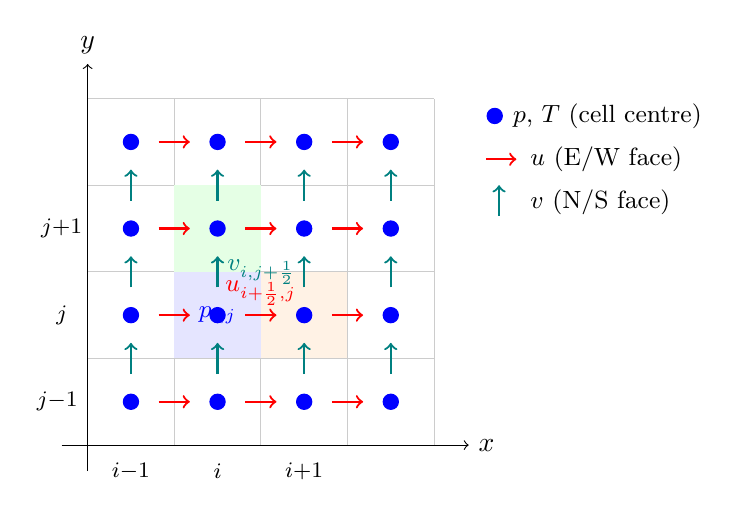
\begin{tikzpicture}[scale=1.1]
    % Grid lines
    \draw[gray!40, thin] (0,0) grid (4,4);

    % Highlight one control volume for p
    \fill[blue!10] (1,1) rectangle (2,2);
    \fill[green!10] (1,2) rectangle (2,3);
    \fill[orange!10] (2,1) rectangle (3,2);

    % Cell centers (pressure / scalar)
    \foreach \i in {0.5,1.5,2.5,3.5} {
        \foreach \j in {0.5,1.5,2.5,3.5} {
            \filldraw[blue] (\i,\j) circle (2.5pt);
        }
    }
    % u-faces (east/west faces)
    \foreach \i in {1,2,3} {
        \foreach \j in {0.5,1.5,2.5,3.5} {
            \draw[red,thick,->] (\i-0.18,\j) -- (\i+0.18,\j);
        }
    }
    % v-faces (north/south faces)
    \foreach \i in {0.5,1.5,2.5,3.5} {
        \foreach \j in {1,2,3} {
            \draw[teal,thick,->] (\i,\j-0.18) -- (\i,\j+0.18);
        }
    }

    % Labels for one cell
    \node[blue, font=\small] at (1.5,1.5) {$p_{i,j}$};
    \node[red,  font=\small, above] at (2,1.5) {$u_{i+\frac{1}{2},j}$};
    \node[teal, font=\small, right] at (1.5,2) {$v_{i,j+\frac{1}{2}}$};

    % Axes
    \draw[->] (-0.3,0) -- (4.4,0) node[right]{$x$};
    \draw[->] (0,-0.3) -- (0,4.4) node[above]{$y$};

    % Index labels
    \node[font=\footnotesize] at (0.5,-0.3) {$i{-}1$};
    \node[font=\footnotesize] at (1.5,-0.3) {$i$};
    \node[font=\footnotesize] at (2.5,-0.3) {$i{+}1$};
    \node[font=\footnotesize] at (-0.35,0.5) {$j{-}1$};
    \node[font=\footnotesize] at (-0.3,1.5) {$j$};
    \node[font=\footnotesize] at (-0.3,2.5) {$j{+}1$};

    % Legend
    \filldraw[blue] (4.7,3.8) circle (2.5pt);
    \node[font=\small, right] at (4.8,3.8) {$p$, $T$ (cell centre)};
    \draw[red,thick,->] (4.6,3.3) -- (4.95,3.3);
    \node[font=\small, right] at (5.0,3.3) {$u$ (E/W face)};
    \draw[teal,thick,->] (4.75,2.65) -- (4.75,3.0);
    \node[font=\small, right] at (5.0,2.8) {$v$ (N/S face)};
\end{tikzpicture}
\caption{Staggered Cartesian grid. Scalars ($p$, $T$) sit at cell centres (blue dots); $u$ is stored on east/west faces (red arrows); $v$ on north/south faces (teal arrows).}
\label{fig:cart_grid}
\end{figure}

% ----------------------------------------------------------
\subsection{Finite Volume Discretisation --- Integration over $\Delta x\,\Delta y$}
% ----------------------------------------------------------

Each equation is integrated over the appropriate control volume (CV) of area $\Delta x\,\Delta y$.

\subsubsection{Continuity Equation}

Integrating Eq.~\eqref{eq:cart_cont} over the scalar CV centred at $(i,j)$:
\begin{equation}
    \int_{\Delta y}\!\int_{\Delta x}
    \left(\frac{\partial u}{\partial x}+\frac{\partial v}{\partial y}\right)
    dx\,dy = 0
\end{equation}

Applying the divergence theorem (face fluxes):
\begin{equation}
    \frac{u_{i+\frac{1}{2},j} - u_{i-\frac{1}{2},j}}{\Delta x}
    + \frac{v_{i,j+\frac{1}{2}} - v_{i,j-\frac{1}{2}}}{\Delta y} = 0
    \label{eq:cart_disc_cont}
\end{equation}

\subsubsection{$x$-Momentum: CV at $(i+\tfrac{1}{2},\,j)$}

Integrating Eq.~\eqref{eq:cart_momx} over $[\,x_i,\,x_{i+1}\,]\times[\,y_{j-\frac{1}{2}},\,y_{j+\frac{1}{2}}\,]$:

\textbf{Temporal term:}
\begin{equation}
    \frac{\partial u_{i+\frac{1}{2},j}}{\partial t} \approx
    \frac{u_{i+\frac{1}{2},j}^{n+1} - u_{i+\frac{1}{2},j}^{n}}{\Delta t}
\end{equation}

\textbf{Convective terms} (central differencing):
\begin{align}
    u\frac{\partial u}{\partial x}\bigg|_{i+\frac{1}{2},j}
    &\approx u_{i+\frac{1}{2},j}\,
       \frac{u_{i+\frac{3}{2},j} - u_{i-\frac{1}{2},j}}{2\,\Delta x}
    \\[4pt]
    v\frac{\partial u}{\partial y}\bigg|_{i+\frac{1}{2},j}
    &\approx \bar{v}_{i+\frac{1}{2},j}\,
       \frac{u_{i+\frac{1}{2},j+1} - u_{i+\frac{1}{2},j-1}}{2\,\Delta y}
\end{align}
where $\bar{v}_{i+\frac{1}{2},j}
= \tfrac{1}{4}\!\left(v_{i,j+\frac{1}{2}}+v_{i+1,j+\frac{1}{2}}
                     +v_{i,j-\frac{1}{2}}+v_{i+1,j-\frac{1}{2}}\right)$
is the averaged $v$ at the $u$-face.

\textbf{Pressure gradient:}
\begin{equation}
    \frac{1}{\rho}\frac{\partial p}{\partial x}\bigg|_{i+\frac{1}{2},j}
    \approx \frac{1}{\rho}\frac{p_{i+1,j} - p_{i,j}}{\Delta x}
\end{equation}

\textbf{Viscous diffusion:}
\begin{equation}
    \nu\!\left(\frac{\partial^2 u}{\partial x^2}
              +\frac{\partial^2 u}{\partial y^2}\right)_{i+\frac{1}{2},j}
    \approx \nu\!\left(
      \frac{u_{i+\frac{3}{2},j}-2u_{i+\frac{1}{2},j}+u_{i-\frac{1}{2},j}}{\Delta x^2}
      +\frac{u_{i+\frac{1}{2},j+1}-2u_{i+\frac{1}{2},j}+u_{i+\frac{1}{2},j-1}}{\Delta y^2}
    \right)
\end{equation}

\subsubsection{$y$-Momentum: CV at $(i,\,j+\tfrac{1}{2})$}

By symmetry with the $x$-momentum equation:

\textbf{Convective terms:}
\begin{align}
    u\frac{\partial v}{\partial x}\bigg|_{i,j+\frac{1}{2}}
    &\approx \bar{u}_{i,j+\frac{1}{2}}\,
       \frac{v_{i+1,j+\frac{1}{2}} - v_{i-1,j+\frac{1}{2}}}{2\,\Delta x}
    \\[4pt]
    v\frac{\partial v}{\partial y}\bigg|_{i,j+\frac{1}{2}}
    &\approx v_{i,j+\frac{1}{2}}\,
       \frac{v_{i,j+\frac{3}{2}} - v_{i,j-\frac{1}{2}}}{2\,\Delta y}
\end{align}
where $\bar{u}_{i,j+\frac{1}{2}}
= \tfrac{1}{4}\!\left(u_{i+\frac{1}{2},j}+u_{i-\frac{1}{2},j}
                     +u_{i+\frac{1}{2},j+1}+u_{i-\frac{1}{2},j+1}\right)$.

% ----------------------------------------------------------
\subsection{Projection (Pressure-Correction) Method}
% ----------------------------------------------------------

\subsubsection{Step 1 --- Predictor (intermediate velocities $u^*$, $v^*$)}

Advance the momentum equations \emph{without} the pressure gradient:

\begin{equation}
\boxed{
u^{*}_{i+\frac{1}{2},j} = u^n_{i+\frac{1}{2},j}
+ \Delta t\left[
  -u^n_{i+\frac{1}{2},j}\frac{u^n_{i+\frac{3}{2},j}-u^n_{i-\frac{1}{2},j}}{2\Delta x}
  -\bar{v}^n_{i+\frac{1}{2},j}\frac{u^n_{i+\frac{1}{2},j+1}-u^n_{i+\frac{1}{2},j-1}}{2\Delta y}
  +\nu\!\left(
    \frac{u^n_{i+\frac{3}{2},j}-2u^n_{i+\frac{1}{2},j}+u^n_{i-\frac{1}{2},j}}{\Delta x^2}
    +\frac{u^n_{i+\frac{1}{2},j+1}-2u^n_{i+\frac{1}{2},j}+u^n_{i+\frac{1}{2},j-1}}{\Delta y^2}
  \right)
\right]
}
\label{eq:cart_pred_u}
\end{equation}

\begin{equation}
\boxed{
v^{*}_{i,j+\frac{1}{2}} = v^n_{i,j+\frac{1}{2}}
+ \Delta t\left[
  -\bar{u}^n_{i,j+\frac{1}{2}}\frac{v^n_{i+1,j+\frac{1}{2}}-v^n_{i-1,j+\frac{1}{2}}}{2\Delta x}
  -v^n_{i,j+\frac{1}{2}}\frac{v^n_{i,j+\frac{3}{2}}-v^n_{i,j-\frac{1}{2}}}{2\Delta y}
  +\nu\!\left(
    \frac{v^n_{i+1,j+\frac{1}{2}}-2v^n_{i,j+\frac{1}{2}}+v^n_{i-1,j+\frac{1}{2}}}{\Delta x^2}
    +\frac{v^n_{i,j+\frac{3}{2}}-2v^n_{i,j+\frac{1}{2}}+v^n_{i,j-\frac{1}{2}}}{\Delta y^2}
  \right)
\right]
}
\label{eq:cart_pred_v}
\end{equation}

\subsubsection{Step 2 --- Poisson Equation for Pressure Correction $p'$}

Enforcing $\nabla\cdot\mathbf{u}^{n+1}=0$ after the corrector step
$\mathbf{u}^{n+1}=\mathbf{u}^*-\Delta t\,\nabla p'/\rho$
yields the Poisson equation:

\begin{equation}
    \frac{\partial^2 p'}{\partial x^2}+\frac{\partial^2 p'}{\partial y^2}
    = \frac{\rho}{\Delta t}\left(
        \frac{\partial u^*}{\partial x}+\frac{\partial v^*}{\partial y}
      \right)
    \label{eq:cart_poisson}
\end{equation}

Discretised on the scalar CV at $(i,j)$:

\begin{equation}
\boxed{
\frac{p'_{i+1,j}-2p'_{i,j}+p'_{i-1,j}}{\Delta x^2}
+\frac{p'_{i,j+1}-2p'_{i,j}+p'_{i,j-1}}{\Delta y^2}
= \frac{\rho}{\Delta t}\left(
  \frac{u^*_{i+\frac{1}{2},j}-u^*_{i-\frac{1}{2},j}}{\Delta x}
  +\frac{v^*_{i,j+\frac{1}{2}}-v^*_{i,j-\frac{1}{2}}}{\Delta y}
\right)
}
\label{eq:cart_disc_poisson}
\end{equation}

This linear system $\mathbf{A}\,\mathbf{p}'=\mathbf{b}$ is solved at every time step (see Section~\ref{sec:cart_poisson_solver}).

\subsubsection{Step 3 --- Velocity Correction}

\begin{equation}
\boxed{
    u^{n+1}_{i+\frac{1}{2},j} = u^*_{i+\frac{1}{2},j}
    - \frac{\Delta t}{\rho}\,\frac{p'_{i+1,j}-p'_{i,j}}{\Delta x}
}
\label{eq:cart_corr_u}
\end{equation}

\begin{equation}
\boxed{
    v^{n+1}_{i,j+\frac{1}{2}} = v^*_{i,j+\frac{1}{2}}
    - \frac{\Delta t}{\rho}\,\frac{p'_{i,j+1}-p'_{i,j}}{\Delta y}
}
\label{eq:cart_corr_v}
\end{equation}

\subsubsection{Step 4 --- Pressure Update}

\begin{equation}
\boxed{
    p^{n+1}_{i,j} = p^{n}_{i,j} + \zeta\,p'_{i,j}
}
\label{eq:cart_pupdate}
\end{equation}

where $\zeta \in (0,1]$ is an under-relaxation factor (commonly $\zeta = 0.5$).

% ----------------------------------------------------------
\subsection{Poisson Solver Procedure}
\label{sec:cart_poisson_solver}
% ----------------------------------------------------------

Equation~\eqref{eq:cart_disc_poisson} can be rearranged to isolate $p'_{i,j}$:

\begin{equation}
    p'_{i,j} = \frac{1}{2\!\left(\dfrac{1}{\Delta x^2}+\dfrac{1}{\Delta y^2}\right)}
    \left[
        \frac{p'_{i+1,j}+p'_{i-1,j}}{\Delta x^2}
       +\frac{p'_{i,j+1}+p'_{i,j-1}}{\Delta y^2}
       - b_{i,j}
    \right]
    \label{eq:cart_gs}
\end{equation}

where
$b_{i,j} = \dfrac{\rho}{\Delta t}
\!\left(\dfrac{u^*_{i+\frac{1}{2},j}-u^*_{i-\frac{1}{2},j}}{\Delta x}
        +\dfrac{v^*_{i,j+\frac{1}{2}}-v^*_{i,j-\frac{1}{2}}}{\Delta y}\right)$.

\textbf{Iterative procedure (Gauss--Seidel or SOR):}
\begin{enumerate}
    \item Initialise $p'_{i,j}=0$ everywhere.
    \item Apply boundary conditions for $p'$ (Neumann $\partial p'/\partial n = 0$ at walls; $p'=0$ at outflow).
    \item Sweep all interior cells using Eq.~\eqref{eq:cart_gs}: \\
          SOR version: $p'^{\,\text{new}}_{i,j} = p'^{\,\text{old}}_{i,j} + \omega\!\left(p'^{\,\text{GS}}_{i,j}-p'^{\,\text{old}}_{i,j}\right)$, with $1 < \omega < 2$.
    \item Check convergence: $\max_{i,j}|p'^{\,\text{new}}_{i,j}-p'^{\,\text{old}}_{i,j}| < \varepsilon$.
    \item Repeat from step 2 until converged.
\end{enumerate}

\textbf{Alternatively --- Direct solver (LU / sparse):}
Assemble the $(N_x N_y)\times(N_x N_y)$ sparse matrix $\mathbf{A}$ from Eq.~\eqref{eq:cart_disc_poisson} and solve $\mathbf{A}\mathbf{p}'=\mathbf{b}$ once per time step using \texttt{scipy.sparse.linalg.spsolve} (or similar).

% ----------------------------------------------------------
\subsection{Ghost Cells and Boundary Conditions}
% ----------------------------------------------------------

Ghost (halo) cells are fictitious cells added one layer outside the physical boundary.  They allow interior-stencil formulas to be applied uniformly up to the boundary without special-casing.

\begin{figure}[H]
\centering
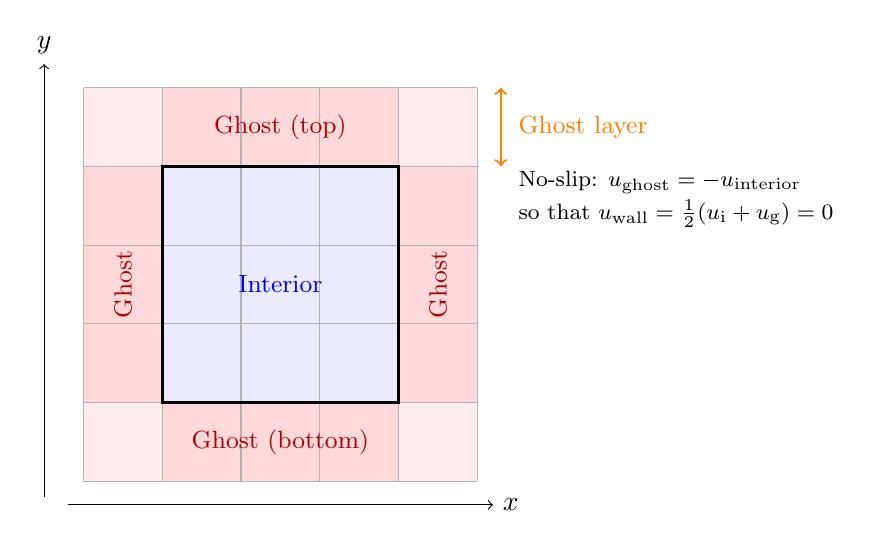
\begin{tikzpicture}[scale=1.0]
    % Physical domain (3x3 interior)
    \fill[blue!8] (1,0) rectangle (4,3);
    % Ghost cells top
    \fill[red!15] (1,3) rectangle (4,4);
    % Ghost cells bottom
    \fill[red!15] (1,-1) rectangle (4,0);
    % Ghost cells left
    \fill[red!15] (0,0) rectangle (1,3);
    % Ghost cells right
    \fill[red!15] (4,0) rectangle (5,3);
    % Ghost corners
    \fill[red!8] (0,-1) rectangle (1,0);
    \fill[red!8] (4,-1) rectangle (5,0);
    \fill[red!8] (0,3) rectangle (1,4);
    \fill[red!8] (4,3) rectangle (5,4);

    % Grid lines
    \draw[gray!60] (0,-1) grid (5,4);
    % Bold boundary
    \draw[black, very thick] (1,0) rectangle (4,3);

    % Labels
    \node[font=\small, blue] at (2.5,1.5) {Interior};
    \node[font=\small, red!70!black] at (2.5,3.5) {Ghost (top)};
    \node[font=\small, red!70!black] at (2.5,-0.5) {Ghost (bottom)};
    \node[font=\small, red!70!black, rotate=90] at (0.5,1.5) {Ghost};
    \node[font=\small, red!70!black, rotate=90] at (4.5,1.5) {Ghost};

    % BC annotation: no-slip wall at top
    \draw[<->, orange, thick] (5.3,3) -- (5.3,4);
    \node[orange, font=\small, right] at (5.4,3.5) {Ghost layer};
    \node[font=\footnotesize, right] at (5.4,2.8) {No-slip: $u_\text{ghost}=-u_\text{interior}$};
    \node[font=\footnotesize, right] at (5.4,2.4) {so that $u_\text{wall}=\tfrac{1}{2}(u_\text{i}+u_\text{g})=0$};

    % Axes
    \draw[->] (-0.2,-1.3) -- (5.2,-1.3) node[right]{$x$};
    \draw[->] (-0.5,-1.2) -- (-0.5,4.3) node[above]{$y$};
\end{tikzpicture}
\caption{Ghost cell (halo) layout for a 2D Cartesian domain. Red cells are ghost cells; blue cells are physical interior cells. The bold rectangle marks the physical boundary.}
\label{fig:cart_ghost}
\end{figure}

\textbf{How to set ghost cell values:}

\begin{center}
\begin{tabular}{llll}
\toprule
Boundary & Condition & Variable & Ghost cell value \\
\midrule
No-slip wall  & $u_w=0$, $v_w=0$  & $u$  & $u_\text{ghost} = -u_\text{interior}$ \\
              &                   & $v$  & $v_\text{ghost} = -v_\text{interior}$ \\
              & $\partial p/\partial n=0$ & $p$ & $p_\text{ghost} = p_\text{interior}$ \\
\midrule
Symmetry (e.g.\ centreline) & $\partial u/\partial y=0$ & $u$ & $u_\text{ghost} = u_\text{interior}$ \\
                             & $v=0$ & $v$ & $v_\text{ghost} = -v_\text{interior}$ \\
\midrule
Inlet & $u=U_\text{in}$, $v=0$ & $u$ & $u_\text{ghost} = 2U_\text{in}-u_\text{interior}$ \\
\midrule
Outlet (zero-gradient) & $\partial(\cdot)/\partial x=0$ & any & $\phi_\text{ghost}=\phi_\text{interior}$ \\
\bottomrule
\end{tabular}
\end{center}

The ghost cell value is computed \emph{before} each Runge--Kutta or Adams--Bashforth stage so that boundary conditions are enforced at the correct sub-step.


% ============================================================
%  Derivation: 2D Cylindrical Coordinates (r, z)
%  Velocities: u (radial), w (axial)
%  Integration element: dr dz   (axisymmetric: no phi dependence)
% ============================================================

\section{2D Incompressible Flow in Cylindrical Coordinates $(r,z)$ --- Velocities $(u,w)$}
\label{sec:cyl_uw}

\emph{Note on notation:} this appendix derives the FVM discretisation, projection method,
and ghost-cell treatment in general form, illustrating $u$ and $w$ as cell-centred quantities
near each boundary for schematic clarity. The staggered grid actually implemented (Table~2 in
the main text) instead stores $u$ exactly \emph{at} the axis and wall faces and $w$ exactly
\emph{at} the inlet and outlet faces, so those boundary-normal components are set directly
(Dirichlet) rather than via a mirrored ghost cell; only the wall-tangential component and the
scalars ($p$, $\theta$) use the mirrored ghost-cell form shown here. The relaxation factor
$\zeta$ below is the same quantity as $\alpha_p$ in Section~\ref{sec:pressure-correction},
where this submission uses $\alpha_p = 0.7$.

\subsection{Governing Equations (Strong Form)}

For axisymmetric flow ($\partial/\partial\phi = 0$, $v_\phi = 0$) in cylindrical coordinates $(r,z)$:

\textbf{Continuity:}
\begin{equation}
    \frac{1}{r}\frac{\partial(ru)}{\partial r}+\frac{\partial w}{\partial z}
    = 0
    \label{eq:cyl_uw_cont}
\end{equation}

\textbf{Radial momentum ($r$-direction):}
\begin{equation}
    \frac{\partial u}{\partial t}
    + \frac{1}{r}\frac{\partial(ru^2)}{\partial r}
    + \frac{\partial(uw)}{\partial z}
    = -\frac{1}{\rho}\frac{\partial p}{\partial r}
    + \frac{1}{\rho r}\frac{\partial(r\tau_{rr})}{\partial r}
    + \frac{1}{\rho}\frac{\partial\tau_{rz}}{\partial z}
    \label{eq:cyl_uw_momr}
\end{equation}

\textbf{Axial momentum ($z$-direction):}
\begin{equation}
    \frac{\partial w}{\partial t}
    + \frac{1}{r}\frac{\partial(ruw)}{\partial r}
    + \frac{\partial(w^2)}{\partial z}
    = -\frac{1}{\rho}\frac{\partial p}{\partial z}
    + \frac{1}{\rho r}\frac{\partial(r\tau_{rz})}{\partial r}
    + \frac{1}{\rho}\frac{\partial\tau_{zz}}{\partial z}
    \label{eq:cyl_uw_momz}
\end{equation}

where for a Newtonian fluid with constant viscosity $\mu = \rho\nu$:
\begin{align}
    \tau_{rr} &= 2\mu\frac{\partial u}{\partial r}
    \\
    \tau_{zz} &= 2\mu\frac{\partial w}{\partial z}
    \\
    \tau_{rz} &= \mu\!\left(\frac{\partial u}{\partial z}+\frac{\partial w}{\partial r}\right)
\end{align}

% ----------------------------------------------------------
\subsection{Staggered Grid Layout}
% ----------------------------------------------------------

\begin{figure}[H]
\centering
\begin{tikzpicture}[scale=1.5, >=Latex]

% ---------------------------------------------------------------
% Front face (theta = theta_j): the (r,z) cross-section of one CV
% ---------------------------------------------------------------
\coordinate (A) at (0,0);       % r_i,     z_j
\coordinate (B) at (2.6,0);     % r_i,     z_{j+1}
\coordinate (C) at (2.6,1.8);   % r_{i+1}, z_{j+1}
\coordinate (D) at (0,1.8);     % r_{i+1}, z_j

% Sweep (theta-direction) offsets. Larger radius -> larger projected
% displacement for the same physical d(theta), since arc length = r*dtheta.
\coordinate (dIn)  at (0.70,0.42);
\coordinate (dOut) at (1.10,0.66);

\coordinate (Ap) at ($(A)+(dIn)$);
\coordinate (Bp) at ($(B)+(dIn)$);
\coordinate (Cp) at ($(C)+(dOut)$);
\coordinate (Dp) at ($(D)+(dOut)$);

% ---- back (hidden) rectangle ----
\draw[gray!55,thin] (Ap) -- (Bp) -- (Cp) -- (Dp) -- cycle;

% ---- sweep edges: r=const cylindrical surfaces, drawn as gentle arcs ----
\draw[gray!65,thin]  (A) to[bend left=8]  (Ap);
\draw[gray!65,thin]  (B) to[bend left=8]  (Bp);
\draw[black!75,thin] (D) to[bend left=14] (Dp);
\draw[black!75,thin] (C) to[bend left=14] (Cp);

% ---- front face: the control volume, highlighted ----
\fill[green!22] (A) -- (B) -- (C) -- (D) -- cycle;
\draw[black,very thick] (A) -- (B) -- (C) -- (D) -- cycle;

% ---- scalar node p,T at cell centre ----
\coordinate (P) at ($(A)!0.5!(C)$);
\filldraw[blue] (P) circle (2.2pt);
\node[blue,font=\small,above right=1pt] at (P) {$p_{i,j},\,T_{i,j}$};

% ---- u (radial velocity) on the r-faces, red -- both point in +r ----
\coordinate (uIn)  at ($(A)!0.5!(B)$);
\coordinate (uOut) at ($(D)!0.5!(C)$);
\draw[red,thick,->] ($(uIn)+(0,-0.22)$)  -- ($(uIn)+(0,0.20)$);
\node[red,font=\small,below] at ($(uIn)+(0,-0.24)$) {$u_{i-\frac12,j}$};
\draw[red,thick,->] ($(uOut)+(0,-0.20)$) -- ($(uOut)+(0,0.22)$);
\node[red,font=\small,above] at ($(uOut)+(0,0.24)$) {$u_{i+\frac12,j}$};

% ---- w (axial velocity) on the z-faces, teal -- both point in +z ----
\coordinate (wLeft)  at ($(A)!0.5!(D)$);
\coordinate (wRight) at ($(B)!0.5!(C)$);
\draw[teal,thick,->] ($(wLeft)+(-0.20,0)$)  -- ($(wLeft)+(0.22,0)$);
\node[teal,font=\small,left] at ($(wLeft)+(-0.22,0)$) {$w_{i,j-\frac12}$};
\draw[teal,thick,->] ($(wRight)+(-0.22,0)$) -- ($(wRight)+(0.20,0)$);
\node[teal,font=\small,right] at ($(wRight)+(0.22,0)$) {$w_{i,j+\frac12}$};

% ---- r_i, r_{i+1} labels with leader lines to the curved (r=const) edges ----
\draw[gray!70] (-0.55,-0.55) -- ($(A)!0.5!(Ap)$);
\node[font=\small] at (-0.75,-0.7) {$r_i$};

\draw[gray!70] (-0.55,2.35) -- ($(D)!0.5!(Dp)$);
\node[font=\small] at (-0.75,2.5) {$r_{i+1}$};

% ---- z_j, z_{j+1} labels ----
\node[font=\small] at (0,-0.35) {$z_j$};
\node[font=\small] at (2.6,-0.35) {$z_{j+1}$};

% ---- dr, dz dimension arrows ----
\draw[<->] (-1.15,0) -- (-1.15,1.8) node[midway,left,font=\small] {$\Delta r$};
\draw[<->] (0,-0.85) -- (2.6,-0.85) node[midway,below,font=\small] {$\Delta z$};

% ---- d(theta) angle indicator on the outer sweep (right of the CV, clear of labels) ----
\draw[purple!70,densely dashed] (C) -- ($(C)+(1.0,0)$);
\draw[purple!70,densely dashed] (Cp) -- ($(C)+(1.0,0)$);
\draw[purple!70] ($(C)+(0.55,0)$) arc[start angle=0, end angle=31, radius=0.55];
\node[purple!70,font=\small] at ($(C)+(0.85,0.22)$) {$\Delta\theta$};

% ---- small r,z,theta orientation triad ----
\begin{scope}[shift={(4.6,0.2)}]
    \draw[->] (0,0) -- (0,0.7) node[above]{$r$};
    \draw[->] (0,0) -- (0.9,0) node[right]{$z$};
    \draw[->] (0,0) to[bend left=25] (0.35,0.32) node[right]{$\theta$};
\end{scope}

% ---- legend ----
\begin{scope}[shift={(4.4,1.55)}]
    \filldraw[blue] (0,0.55) circle (2.2pt);
    \node[font=\small,right] at (0.15,0.55) {$p,\,T$ (cell centre)};
    \draw[red,thick,->] (0,0.15) -- (0,0.4);
    \node[font=\small,right] at (0.15,0.28) {$u$ ($r$-face)};
    \draw[teal,thick,->] (0,-0.15) -- (0.25,-0.15);
    \node[font=\small,right] at (0.35,-0.15) {$w$ ($z$-face)};
\end{scope}

\end{tikzpicture}
\caption{Staggered grid in the $(r,z)$ plane. Scalars ($p$, $T$) at the cell centre
         (blue); radial velocity $u$ on the (curved, cylindrical) $r$-faces (red);
         axial velocity $w$ on the $z$-faces (teal). The control volume is drawn
         swept through a finite $\Delta\theta$ purely to convey the 3-D cylindrical
         shape of the $r$-faces (note the outer face at $r_{i+1}$ sweeps further
         than the inner face at $r_i$, since arc length $=r\,\Delta\theta$); the
         axisymmetric problem itself has $\partial/\partial\theta = 0$ and no
         $\theta$-dependence.}
\label{fig:cyl_uw_grid}
\end{figure}

% ----------------------------------------------------------
\subsection{Finite Volume Discretisation --- Integration over $\Delta r\,\Delta z$}
% ----------------------------------------------------------

The volume element for an axisymmetric ring CV is $dV = r\,dr\,d\phi\,dz$.
After integrating over $\phi\in[0,2\pi]$, every integral acquires the factor $2\pi$.
Since the same factor appears on both sides of the momentum equations, it cancels and we work with the \emph{area} element $r\,dr\,dz$.

\subsubsection{Continuity Equation}

Integrate Eq.~\eqref{eq:cyl_uw_cont} over the scalar CV
$[r_{i-\frac{1}{2}},r_{i+\frac{1}{2}}]\times[z_{j-\frac{1}{2}},z_{j+\frac{1}{2}}]$:
\begin{equation}
    \int_{r_{i-\frac{1}{2}}}^{r_{i+\frac{1}{2}}}
    \int_{z_{j-\frac{1}{2}}}^{z_{j+\frac{1}{2}}}
    \left[\frac{1}{r}\frac{\partial(ru)}{\partial r}+\frac{\partial w}{\partial z}\right]
    r\,dr\,dz = 0
\end{equation}

Applying the FV divergence theorem:
\begin{equation}
\boxed{
    \frac{r_{i+\frac{1}{2}}\,u_{i+\frac{1}{2},j} - r_{i-\frac{1}{2}}\,u_{i-\frac{1}{2},j}}{r_i\,\Delta r}
    + \frac{w_{i,j+\frac{1}{2}} - w_{i,j-\frac{1}{2}}}{\Delta z} = 0
}
\label{eq:cyl_uw_disc_cont}
\end{equation}

\subsubsection{Axial Momentum: CV at $(i,\,j+\tfrac{1}{2})$}

Integrate Eq.~\eqref{eq:cyl_uw_momz} over $[r_{i-\frac{1}{2}},r_{i+\frac{1}{2}}]\times[z_j,z_{j+1}]$,
weighting by $r$:

\textbf{Temporal term:}
\begin{equation}
    \frac{\partial w_{i,j+\frac{1}{2}}}{\partial t}
    \approx \frac{w_{i,j+\frac{1}{2}}^{n+1}-w_{i,j+\frac{1}{2}}^{n}}{\Delta t}
\end{equation}

\textbf{Convective terms:}
\begin{align}
    u\frac{\partial w}{\partial r}\bigg|_{i,j+\frac{1}{2}}
    &\approx \bar{u}_{i,j+\frac{1}{2}}\,
      \frac{w_{i+1,j+\frac{1}{2}}-w_{i-1,j+\frac{1}{2}}}{2\Delta r}
    \\[4pt]
    w\frac{\partial w}{\partial z}\bigg|_{i,j+\frac{1}{2}}
    &\approx w_{i,j+\frac{1}{2}}\,
      \frac{w_{i,j+\frac{3}{2}}-w_{i,j-\frac{1}{2}}}{2\Delta z}
\end{align}
where $\bar{u}_{i,j+\frac{1}{2}}
= \tfrac{1}{4}(u_{i+\frac{1}{2},j}+u_{i-\frac{1}{2},j}
              +u_{i+\frac{1}{2},j+1}+u_{i-\frac{1}{2},j+1})$.

\textbf{Pressure gradient:}
\begin{equation}
    \frac{1}{\rho}\frac{\partial p}{\partial z}\bigg|_{i,j+\frac{1}{2}}
    \approx \frac{1}{\rho}\frac{p_{i,j+1}-p_{i,j}}{\Delta z}
\end{equation}

\textbf{Viscous diffusion (using $\frac{1}{r}\frac{\partial}{\partial r}(r\frac{\partial w}{\partial r})$):}
\begin{align}
    \nu\!\left(\frac{\partial^2 w}{\partial r^2}+\frac{1}{r}\frac{\partial w}{\partial r}\right)
    &\approx \frac{\nu}{r_i\Delta r}\left(
       r_{i+\frac{1}{2}}\frac{w_{i+1,j+\frac{1}{2}}-w_{i,j+\frac{1}{2}}}{\Delta r}
      -r_{i-\frac{1}{2}}\frac{w_{i,j+\frac{1}{2}}-w_{i-1,j+\frac{1}{2}}}{\Delta r}
    \right)
    \\[4pt]
    \nu\frac{\partial^2 w}{\partial z^2}
    &\approx \nu\frac{w_{i,j+\frac{3}{2}}-2w_{i,j+\frac{1}{2}}+w_{i,j-\frac{1}{2}}}{\Delta z^2}
\end{align}

\subsubsection{Radial Momentum: CV at $(i+\tfrac{1}{2},\,j)$}

Integrate Eq.~\eqref{eq:cyl_uw_momr} over $[r_i,r_{i+1}]\times[z_{j-\frac{1}{2}},z_{j+\frac{1}{2}}]$:

\textbf{Convective terms:}
\begin{align}
    u\frac{\partial u}{\partial r}\bigg|_{i+\frac{1}{2},j}
    &\approx u_{i+\frac{1}{2},j}\,
      \frac{u_{i+\frac{3}{2},j}-u_{i-\frac{1}{2},j}}{2\Delta r}
    \\[4pt]
    w\frac{\partial u}{\partial z}\bigg|_{i+\frac{1}{2},j}
    &\approx \bar{w}_{i+\frac{1}{2},j}\,
      \frac{u_{i+\frac{1}{2},j+1}-u_{i+\frac{1}{2},j-1}}{2\Delta z}
\end{align}

\textbf{Pressure gradient:}
\begin{equation}
    \frac{1}{\rho}\frac{\partial p}{\partial r}\bigg|_{i+\frac{1}{2},j}
    \approx \frac{1}{\rho}\frac{p_{i+1,j}-p_{i,j}}{\Delta r}
\end{equation}

\textbf{Viscous diffusion:}
\begin{align}
    \nu\!\left(\frac{\partial^2 u}{\partial r^2}+\frac{1}{r}\frac{\partial u}{\partial r}-\frac{u}{r^2}\right)
    &\approx \frac{\nu}{r_{i+\frac{1}{2}}\Delta r}\left(
       r_{i+1}\frac{u_{i+\frac{3}{2},j}-u_{i+\frac{1}{2},j}}{\Delta r}
      -r_i\frac{u_{i+\frac{1}{2},j}-u_{i-\frac{1}{2},j}}{\Delta r}
    \right) - \frac{\nu\,u_{i+\frac{1}{2},j}}{r_{i+\frac{1}{2}}^2}
    \\[4pt]
    \nu\frac{\partial^2 u}{\partial z^2}
    &\approx \nu\frac{u_{i+\frac{1}{2},j+1}-2u_{i+\frac{1}{2},j}+u_{i+\frac{1}{2},j-1}}{\Delta z^2}
\end{align}

% ----------------------------------------------------------
\subsection{Projection Method}
% ----------------------------------------------------------

\subsubsection{Step 1 --- Predictor}

Advance without the pressure gradient (explicit Euler or AB2):

\begin{equation}
\boxed{
w^{*}_{i,j+\frac{1}{2}} = w^n_{i,j+\frac{1}{2}} + \Delta t\,\Bigl[
  -\bar{u}^n\,\frac{w^n_{i+1,j+\frac{1}{2}}-w^n_{i-1,j+\frac{1}{2}}}{2\Delta r}
  -w^n_{i,j+\frac{1}{2}}\,\frac{w^n_{i,j+\frac{3}{2}}-w^n_{i,j-\frac{1}{2}}}{2\Delta z}
  +\nu D_r^w + \nu D_z^w
\Bigr]
}
\label{eq:cyl_uw_pred_w}
\end{equation}

\begin{equation}
\boxed{
u^{*}_{i+\frac{1}{2},j} = u^n_{i+\frac{1}{2},j} + \Delta t\,\Bigl[
  -u^n_{i+\frac{1}{2},j}\,\frac{u^n_{i+\frac{3}{2},j}-u^n_{i-\frac{1}{2},j}}{2\Delta r}
  -\bar{w}^n\,\frac{u^n_{i+\frac{1}{2},j+1}-u^n_{i+\frac{1}{2},j-1}}{2\Delta z}
  +\nu D_r^u + \nu D_z^u
\Bigr]
}
\label{eq:cyl_uw_pred_u}
\end{equation}

where the diffusion operators are:
\begin{align}
    D_r^w &= \frac{1}{r_i\Delta r}\!\left(
       r_{i+\frac{1}{2}}\frac{w^n_{i+1,j+\frac{1}{2}}-w^n_{i,j+\frac{1}{2}}}{\Delta r}
      -r_{i-\frac{1}{2}}\frac{w^n_{i,j+\frac{1}{2}}-w^n_{i-1,j+\frac{1}{2}}}{\Delta r}
    \right),\quad
    D_z^w = \frac{w^n_{i,j+\frac{3}{2}}-2w^n_{i,j+\frac{1}{2}}+w^n_{i,j-\frac{1}{2}}}{\Delta z^2}
    \\[4pt]
    D_r^u &= \frac{r_{i+1}(u^n_{i+\frac{3}{2},j}-u^n_{i+\frac{1}{2},j})-r_i(u^n_{i+\frac{1}{2},j}-u^n_{i-\frac{1}{2},j})}{r_{i+\frac{1}{2}}\Delta r^2}
    - \frac{u^n_{i+\frac{1}{2},j}}{r_{i+\frac{1}{2}}^2}
    \\[4pt]
    D_z^u &= \frac{u^n_{i+\frac{1}{2},j+1}-2u^n_{i+\frac{1}{2},j}+u^n_{i+\frac{1}{2},j-1}}{\Delta z^2}
\end{align}

\subsubsection{Step 2 --- Poisson Equation for Pressure Correction $p'$}

Enforcing the discrete continuity Eq.~\eqref{eq:cyl_uw_disc_cont} after correction:
\begin{equation}
    \frac{1}{r}\frac{\partial}{\partial r}\!\left(r\frac{\partial p'}{\partial r}\right)
    +\frac{\partial^2 p'}{\partial z^2}
    = \frac{\rho}{\Delta t}\left(
       \frac{1}{r}\frac{\partial(ru^*)}{\partial r}+\frac{\partial w^*}{\partial z}
      \right)
\end{equation}

Discretised form at cell $(i,j)$:
\begin{equation}
\resizebox{\textwidth}{!}{$\displaystyle
\boxed{
\frac{r_{i+\frac{1}{2}}(p'_{i+1,j}-p'_{i,j}) - r_{i-\frac{1}{2}}(p'_{i,j}-p'_{i-1,j})}{r_i\,\Delta r^2}
+\frac{p'_{i,j+1}-2p'_{i,j}+p'_{i,j-1}}{\Delta z^2}
= \frac{\rho}{\Delta t}\left(
  \frac{r_{i+\frac{1}{2}}\,u^*_{i+\frac{1}{2},j}-r_{i-\frac{1}{2}}\,u^*_{i-\frac{1}{2},j}}{r_i\,\Delta r}
  +\frac{w^*_{i,j+\frac{1}{2}}-w^*_{i,j-\frac{1}{2}}}{\Delta z}
\right)
}$}
\label{eq:cyl_uw_disc_poisson}
\end{equation}

\subsubsection{Step 3 --- Velocity Correction}

\begin{equation}
\boxed{
    w^{n+1}_{i,j+\frac{1}{2}} = w^*_{i,j+\frac{1}{2}}
    - \frac{\Delta t}{\rho}\,\frac{p'_{i,j+1}-p'_{i,j}}{\Delta z}
}
\label{eq:cyl_uw_corr_w}
\end{equation}

\begin{equation}
\boxed{
    u^{n+1}_{i+\frac{1}{2},j} = u^*_{i+\frac{1}{2},j}
    - \frac{\Delta t}{\rho}\,\frac{p'_{i+1,j}-p'_{i,j}}{\Delta r}
}
\label{eq:cyl_uw_corr_u}
\end{equation}

\subsubsection{Step 4 --- Pressure Update}

\begin{equation}
\boxed{
    p^{n+1}_{i,j} = p^{n}_{i,j} + \zeta\,p'_{i,j}, \qquad \zeta = \alpha_p = 0.7 \text{ (this submission)}
}
\label{eq:cyl_uw_pupdate}
\end{equation}

% ----------------------------------------------------------
\subsection{Poisson Solver Procedure}
% ----------------------------------------------------------

Rearranging Eq.~\eqref{eq:cyl_uw_disc_poisson} to isolate $p'_{i,j}$:
\begin{equation}
    p'_{i,j} = \frac{b_{i,j} -
      \dfrac{r_{i+\frac{1}{2}}\,p'_{i+1,j}+r_{i-\frac{1}{2}}\,p'_{i-1,j}}{r_i\,\Delta r^2}
      -\dfrac{p'_{i,j+1}+p'_{i,j-1}}{\Delta z^2}
    }
    {-\dfrac{r_{i+\frac{1}{2}}+r_{i-\frac{1}{2}}}{r_i\,\Delta r^2}
     -\dfrac{2}{\Delta z^2}}
    \label{eq:cyl_uw_gs}
\end{equation}

\textbf{Gauss--Seidel / SOR iteration:}
\begin{enumerate}
    \item Set $p'=0$ everywhere.
    \item Enforce BCs: $\partial p'/\partial r=0$ at wall \& centreline; $\partial p'/\partial z=0$ at inlet/outlet (or $p'=0$ at outlet).
    \item Sweep interior cells with Eq.~\eqref{eq:cyl_uw_gs}; apply SOR: $p'^{\text{new}} = p'^{\text{old}}+\omega(p'^{\text{GS}}-p'^{\text{old}})$.
    \item Converge when $\max|p'^{\text{new}}-p'^{\text{old}}|<\varepsilon$.
\end{enumerate}

\textbf{Direct solve:} assemble sparse $\mathbf{A}$ from Eq.~\eqref{eq:cyl_uw_disc_poisson} and call \texttt{spsolve}.
Note: fix one pressure value (e.g.\ $p'_{1,N_z}=0$ at the outlet corner) to remove the null space.

% ----------------------------------------------------------
\subsection{Ghost Cells and Boundary Conditions}
% ----------------------------------------------------------

\begin{figure}[H]
\centering
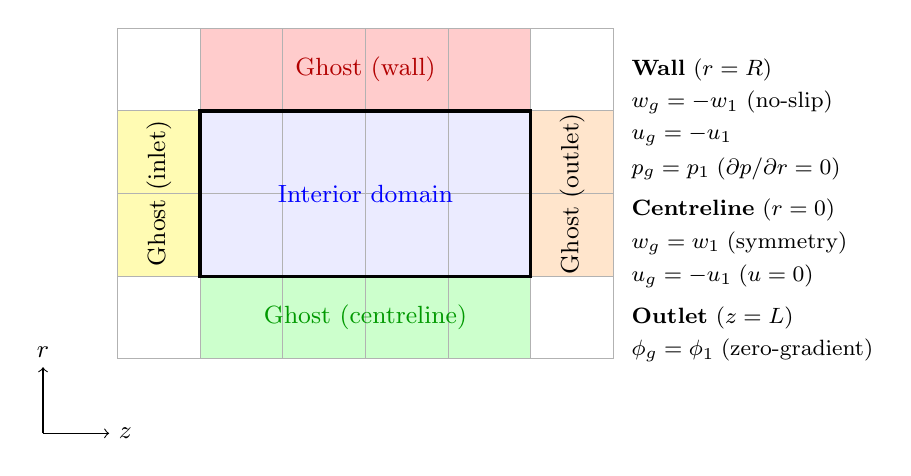
\begin{tikzpicture}[scale=1.05]
    % Physical domain
    \fill[blue!8] (1,1) rectangle (5,3);
    % Ghost: bottom (centreline r=0)
    \fill[green!20] (1,0) rectangle (5,1);
    % Ghost: top (wall r=R)
    \fill[red!20] (1,3) rectangle (5,4);
    % Ghost: left (inlet z=0)
    \fill[yellow!30] (0,1) rectangle (1,3);
    % Ghost: right (outlet z=L)
    \fill[orange!20] (5,1) rectangle (6,3);

    % Grid lines
    \draw[gray!60,thin] (0,0) grid (6,4);
    % Physical boundary
    \draw[black,very thick] (1,1) rectangle (5,3);

    % Arrows / axes -- kept in a clear corner, away from the ghost-band labels
    \draw[->] (-0.9,-0.9) -- (-0.9,-0.1) node[above,font=\small]{$r$};
    \draw[->] (-0.9,-0.9) -- (-0.1,-0.9) node[right,font=\small]{$z$};

    % Labels
    \node[blue,  font=\small] at (3,2)   {Interior domain};
    \node[green!60!black, font=\small] at (3,0.5)   {Ghost (centreline)};
    \node[red!70!black,   font=\small] at (3,3.5)   {Ghost (wall)};
    \node[font=\small, rotate=90] at (0.5,2)  {Ghost (inlet)};
    \node[font=\small, rotate=90] at (5.5,2) {Ghost (outlet)};

    % BC notes
    \node[font=\footnotesize, right] at (6.1,3.5) {\textbf{Wall} ($r=R$)};
    \node[font=\footnotesize, right] at (6.1,3.1) {$w_g = -w_1$ (no-slip)};
    \node[font=\footnotesize, right] at (6.1,2.7) {$u_g = -u_1$};
    \node[font=\footnotesize, right] at (6.1,2.3) {$p_g = p_1$\;($\partial p/\partial r=0$)};

    \node[font=\footnotesize, right] at (6.1,1.8) {\textbf{Centreline} ($r=0$)};
    \node[font=\footnotesize, right] at (6.1,1.4) {$w_g = w_1$\;(symmetry)};
    \node[font=\footnotesize, right] at (6.1,1.0) {$u_g = -u_1$\;($u=0$)};

    \node[font=\footnotesize, right] at (6.1,0.5) {\textbf{Outlet} ($z=L$)};
    \node[font=\footnotesize, right] at (6.1,0.1) {$\phi_g = \phi_1$\;(zero-gradient)};
\end{tikzpicture}
\caption{Ghost cell layout for the $(r,z)$ domain. Green: centreline symmetry; red: no-slip wall; yellow: inlet; orange: outlet. Subscript $g$ = ghost, subscript $1$ = first interior cell.}
\label{fig:cyl_uw_ghost}
\end{figure}

\begin{center}
\begin{tabular}{llll}
\toprule
Boundary & Condition & Variable & Ghost value \\
\midrule
Centreline ($r=0$) & $u=0$               & $u$ & $u_g = -u_1$ \\
                   & $\partial w/\partial r=0$ & $w$ & $w_g = w_1$ \\
                   & $\partial p/\partial r=0$ & $p$ & $p_g = p_1$ \\
\midrule
Wall ($r=R$)       & $u=0$, $w=0$        & $u$ & $u_g = -u_1$ \\
                   &                     & $w$ & $w_g = -w_1$ \\
                   & $\partial p/\partial r=0$ & $p$ & $p_g = p_1$ \\
                   & $\lambda\,\partial T/\partial r=q_w$ & $T$ & $T_g = T_1 + \frac{q_w\,\Delta r}{\lambda}$ \\
\midrule
Inlet ($z=0$)      & $u=0$, $w=W_\text{in}$ & $w$ & $w_g = 2W_\text{in}-w_1$ \\
                   &                        & $u$ & $u_g = -u_1$ \\
                   & $T=T_\text{in}$        & $T$ & $T_g = 2T_\text{in}-T_1$ \\
\midrule
Outlet ($z=L$)     & $\partial(\cdot)/\partial z=0$ & any & $\phi_g = \phi_1$ \\
\bottomrule
\end{tabular}
\end{center}


% ============================================================
%  Derivation: 2D Cylindrical Coordinates (r, phi)
%  Velocities: u (radial), v (azimuthal)
%  Integration element: dr dphi   (no z-dependence)
% ============================================================

\section{2D Incompressible Flow in Cylindrical Coordinates $(r,\phi)$ --- Velocities $(u,v)$}
\label{sec:cyl_uv}

\subsection{Governing Equations (Strong Form)}

For flow in the $(r,\phi)$-plane with $\partial/\partial z = 0$ and $w = 0$:

\textbf{Continuity:}
\begin{equation}
    \frac{1}{r}\frac{\partial(ru)}{\partial r}
    +\frac{1}{r}\frac{\partial v}{\partial\phi} = 0
    \quad\Longleftrightarrow\quad
    \frac{\partial u}{\partial r}+\frac{u}{r}
    +\frac{1}{r}\frac{\partial v}{\partial\phi} = 0
    \label{eq:cyl_uv_cont}
\end{equation}

\textbf{Radial momentum ($r$-direction):}
\begin{equation}
    \frac{\partial u}{\partial t}
    + \frac{1}{r}\frac{\partial(ru^2)}{\partial r}
    + \frac{1}{r}\frac{\partial(uv)}{\partial\phi}
    - \frac{v^2}{r}
    = -\frac{1}{\rho}\frac{\partial p}{\partial r}
    + \frac{1}{\rho r}\frac{\partial(r\tau_{rr})}{\partial r}
    + \frac{1}{\rho r}\frac{\partial\tau_{r\phi}}{\partial\phi}
    - \frac{\tau_{\phi\phi}}{\rho r}
    \label{eq:cyl_uv_momr}
\end{equation}

\textbf{Azimuthal momentum ($\phi$-direction):}
\begin{equation}
    \frac{\partial v}{\partial t}
    + \frac{1}{r}\frac{\partial(ruv)}{\partial r}
    + \frac{1}{r}\frac{\partial(v^2)}{\partial\phi}
    + \frac{uv}{r}
    = -\frac{1}{\rho r}\frac{\partial p}{\partial\phi}
    + \frac{1}{\rho r}\frac{\partial(r\tau_{r\phi})}{\partial r}
    + \frac{1}{\rho r}\frac{\partial\tau_{\phi\phi}}{\partial\phi}
    \label{eq:cyl_uv_momv}
\end{equation}

where $\tau_{rr}$, $\tau_{r\phi}$, and $\tau_{\phi\phi}$ are stress tensor components. For Newtonian fluids with constant viscosity $\mu = \rho\nu$:
\begin{align}
    \tau_{rr} &= 2\mu\frac{\partial u}{\partial r}
    \\
    \tau_{r\phi} &= \mu\!\left(r\frac{\partial}{\partial r}\left(\frac{v}{r}\right)+\frac{1}{r}\frac{\partial u}{\partial\phi}\right)
    \\
    \tau_{\phi\phi} &= 2\mu\left(\frac{u}{r}+\frac{1}{r}\frac{\partial v}{\partial\phi}\right)
\end{align}

The centripetal ($-v^2/r$) and Coriolis ($+uv/r$) terms arise from the curvature of the coordinate system.

\textbf{Conservation vs.\ Convective Form:}
The equations above are in \emph{conservation form}, expressing momentum fluxes as divergences: $\frac{1}{r}\frac{\partial(ru^2)}{\partial r}$ and $\frac{1}{r}\frac{\partial(uv)}{\partial\phi}$ in the radial equation. To derive the \emph{convective form}, expand these using the product rule. For example, in the radial momentum equation:
\begin{equation}
    \frac{1}{r}\frac{\partial(ru^2)}{\partial r} + \frac{1}{r}\frac{\partial(uv)}{\partial\phi}
    = \frac{u}{r}\frac{\partial(ru)}{\partial r} + u\frac{\partial u}{\partial r} + \frac{1}{r}\frac{\partial(uv)}{\partial\phi}
    = u\left(\frac{1}{r}\frac{\partial(ru)}{\partial r} + \frac{1}{r}\frac{\partial v}{\partial\phi}\right) + u\frac{\partial u}{\partial r} + \frac{v}{r}\frac{\partial u}{\partial\phi}
\end{equation}
By continuity $\frac{1}{r}\frac{\partial(ru)}{\partial r} + \frac{1}{r}\frac{\partial v}{\partial\phi} = 0$, the grouped term vanishes:
\begin{equation}
    \frac{1}{r}\frac{\partial(ru^2)}{\partial r} + \frac{1}{r}\frac{\partial(uv)}{\partial\phi} = u\frac{\partial u}{\partial r} + \frac{v}{r}\frac{\partial u}{\partial\phi}
\end{equation}
This is the **convective form**. In cylindrical coordinates, the conservation form is essential for finite volume methods because the metric factors ($r$-weighting) appear naturally in the flux integrals. The divergence structure ensures that discrete momentum is conserved when integrated over the annular control volume with area element $r\,dr\,d\phi$.

% ----------------------------------------------------------
\subsection{Staggered Grid Layout}
% ----------------------------------------------------------

\begin{figure}[H]
\centering
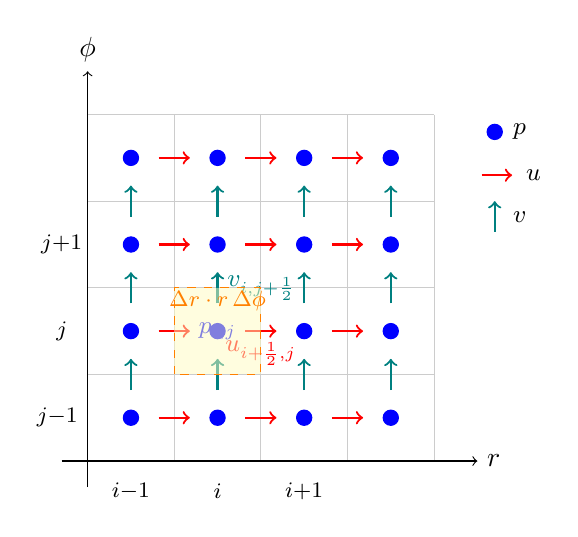
\begin{tikzpicture}[scale=1.1]
    % Grid (r horizontal, phi vertical)
    \draw[gray!40,thin] (0,0) grid (4,4);

    % Cell centres
    \foreach \i in {0.5,1.5,2.5,3.5}{
        \foreach \j in {0.5,1.5,2.5,3.5}{
            \filldraw[blue] (\i,\j) circle (2.5pt);
        }
    }
    % u-faces (radial direction, horizontal faces)
    \foreach \i in {1,2,3}{
        \foreach \j in {0.5,1.5,2.5,3.5}{
            \draw[red,thick,->] (\i-0.18,\j) -- (\i+0.18,\j);
        }
    }
    % v-faces (azimuthal direction, vertical faces)
    \foreach \i in {0.5,1.5,2.5,3.5}{
        \foreach \j in {1,2,3}{
            \draw[teal,thick,->] (\i,\j-0.18) -- (\i,\j+0.18);
        }
    }

    % Axes
    \draw[->] (-0.3,0) -- (4.5,0) node[right]{$r$};
    \draw[->] (0,-0.3) -- (0,4.5) node[above]{$\phi$};

    % Labels for one cell
    \node[blue,  font=\small] at (1.5,1.5) {$p_{i,j}$};
    \node[red,   font=\small, below] at (2,1.5) {$u_{i+\frac{1}{2},j}$};
    \node[teal,  font=\small, right] at (1.5,2) {$v_{i,j+\frac{1}{2}}$};

    % Index labels
    \node[font=\footnotesize] at (0.5,-0.35) {$i{-}1$};
    \node[font=\footnotesize] at (1.5,-0.35) {$i$};
    \node[font=\footnotesize] at (2.5,-0.35) {$i{+}1$};
    \node[font=\footnotesize] at (-0.35,0.5) {$j{-}1$};
    \node[font=\footnotesize] at (-0.3,1.5) {$j$};
    \node[font=\footnotesize] at (-0.3,2.5) {$j{+}1$};

    % Control volume sketch
    \fill[yellow!25, opacity=0.5] (1,1) rectangle (2,2);
    \draw[dashed, orange] (1,1) rectangle (2,2);
    \node[font=\footnotesize, orange] at (1.5,1.85) {$\Delta r \cdot r\,\Delta\phi$};

    % Legend
    \filldraw[blue] (4.7,3.8) circle (2.5pt); \node[font=\small,right] at (4.8,3.8) {$p$};
    \draw[red,thick,->]  (4.55,3.3) -- (4.9,3.3); \node[font=\small,right] at (4.95,3.3) {$u$};
    \draw[teal,thick,->] (4.7,2.65) -- (4.7,3.0); \node[font=\small,right] at (4.8,2.82) {$v$};
\end{tikzpicture}
\caption{Staggered grid in the $(r,\phi)$ plane. Scalars at cell centres (blue); radial velocity $u$ at $r$-faces (red); azimuthal velocity $v$ at $\phi$-faces (teal). The control volume area element is $\Delta r \cdot r\,\Delta\phi$.}
\label{fig:cyl_uv_grid}
\end{figure}

% ----------------------------------------------------------
\subsection{Finite Volume Discretisation --- Integration over $\Delta r\,(r\,\Delta\phi)$}
% ----------------------------------------------------------

The FV approach integrates the conservation laws over a discrete control volume (CV), converting PDEs into algebraic equations. The key tool is the **2D Gauss divergence theorem**:

\begin{equation}
    \iint_{\Omega} \nabla \cdot \mathbf{F} \, dA = \oint_{\partial\Omega} \mathbf{F} \cdot \mathbf{n} \, ds
\end{equation}

where $\Omega$ is the control volume, $\mathbf{F}$ is a flux vector, and $\mathbf{n}$ is the outward normal. This transforms volume integrals of divergence into surface integrals of normal fluxes, which are discretized at cell faces. This is why the **conservation form** of the equations (with divergence operators) is so natural for FV: each divergence term directly corresponds to net flux out of the cell boundaries.

\textbf{Domain:} The FV area element in the $(r,\phi)$-plane is $dA = r\,dr\,d\phi$.
Cell $(i,j)$ occupies $r\in[r_{i-\frac{1}{2}},r_{i+\frac{1}{2}}]$,
$\phi\in[\phi_{j-\frac{1}{2}},\phi_{j+\frac{1}{2}}]$.

\subsubsection{Continuity Equation}

Integrating Eq.~\eqref{eq:cyl_uv_cont} over the scalar CV:
\begin{equation}
    \int_{\phi_{j-\frac{1}{2}}}^{\phi_{j+\frac{1}{2}}}
    \int_{r_{i-\frac{1}{2}}}^{r_{i+\frac{1}{2}}}
    \left[\frac{1}{r}\frac{\partial(ru)}{\partial r}
         +\frac{1}{r}\frac{\partial v}{\partial\phi}\right]
    r\,dr\,d\phi = 0
\end{equation}

Applying the 2D divergence theorem:
\begin{equation}
\boxed{
    \frac{r_{i+\frac{1}{2}}\,u_{i+\frac{1}{2},j} - r_{i-\frac{1}{2}}\,u_{i-\frac{1}{2},j}}{r_i\,\Delta r}
    + \frac{v_{i,j+\frac{1}{2}} - v_{i,j-\frac{1}{2}}}{r_i\,\Delta\phi} = 0
}
\label{eq:cyl_uv_disc_cont}
\end{equation}

\subsubsection{Azimuthal Momentum: CV at $(i,\,j+\tfrac{1}{2})$}

Integrate Eq.~\eqref{eq:cyl_uv_momv} over $[r_{i-\frac{1}{2}},r_{i+\frac{1}{2}}]\times[\phi_j,\phi_{j+1}]$:

\textbf{Temporal term:}
\begin{equation}
    \frac{v_{i,j+\frac{1}{2}}^{n+1}-v_{i,j+\frac{1}{2}}^{n}}{\Delta t}
\end{equation}

\textbf{Convective terms:}
\begin{align}
    u\frac{\partial v}{\partial r}\bigg|_{i,j+\frac{1}{2}}
    &\approx \bar{u}_{i,j+\frac{1}{2}}\,
      \frac{v_{i+1,j+\frac{1}{2}}-v_{i-1,j+\frac{1}{2}}}{2\Delta r}
    \\[4pt]
    \frac{v}{r}\frac{\partial v}{\partial\phi}\bigg|_{i,j+\frac{1}{2}}
    &\approx \frac{v_{i,j+\frac{1}{2}}}{r_i}\,
      \frac{v_{i,j+\frac{3}{2}}-v_{i,j-\frac{1}{2}}}{2\Delta\phi}
    \\[4pt]
    \frac{uv}{r}\bigg|_{i,j+\frac{1}{2}}
    &\approx \frac{\bar{u}_{i,j+\frac{1}{2}}\,v_{i,j+\frac{1}{2}}}{r_i}
    \quad\text{(centripetal coupling term)}
\end{align}

\textbf{Pressure gradient:}
\begin{equation}
    \frac{1}{\rho r}\frac{\partial p}{\partial\phi}\bigg|_{i,j+\frac{1}{2}}
    \approx \frac{1}{\rho\,r_i}\,\frac{p_{i,j+1}-p_{i,j}}{\Delta\phi}
\end{equation}

\textbf{Viscous diffusion:}
\begin{align}
    \nu\!\left(\frac{\partial^2 v}{\partial r^2}+\frac{1}{r}\frac{\partial v}{\partial r}-\frac{v}{r^2}\right)
    &\approx \frac{\nu}{r_i\,\Delta r}\!\left(
       r_{i+\frac{1}{2}}\frac{v_{i+1,j+\frac{1}{2}}-v_{i,j+\frac{1}{2}}}{\Delta r}
      -r_{i-\frac{1}{2}}\frac{v_{i,j+\frac{1}{2}}-v_{i-1,j+\frac{1}{2}}}{\Delta r}
    \right) - \frac{\nu\,v_{i,j+\frac{1}{2}}}{r_i^2}
    \\[4pt]
    \frac{\nu}{r^2}\frac{\partial^2 v}{\partial\phi^2}
    &\approx \frac{\nu}{r_i^2}\,
      \frac{v_{i,j+\frac{3}{2}}-2v_{i,j+\frac{1}{2}}+v_{i,j-\frac{1}{2}}}{\Delta\phi^2}
    \\[4pt]
    \frac{2\nu}{r^2}\frac{\partial u}{\partial\phi}
    &\approx \frac{2\nu}{r_i^2}\,
      \frac{\bar{u}_{i,j+1}-\bar{u}_{i,j}}{\Delta\phi}
\end{align}

\subsubsection{Radial Momentum: CV at $(i+\tfrac{1}{2},\,j)$}

\textbf{Convective terms:}
\begin{align}
    u\frac{\partial u}{\partial r}\bigg|_{i+\frac{1}{2},j}
    &\approx u_{i+\frac{1}{2},j}\,
      \frac{u_{i+\frac{3}{2},j}-u_{i-\frac{1}{2},j}}{2\Delta r}
    \\[4pt]
    \frac{v}{r}\frac{\partial u}{\partial\phi}\bigg|_{i+\frac{1}{2},j}
    &\approx \frac{\bar{v}_{i+\frac{1}{2},j}}{r_{i+\frac{1}{2}}}\,
      \frac{u_{i+\frac{1}{2},j+1}-u_{i+\frac{1}{2},j-1}}{2\Delta\phi}
    \\[4pt]
    \frac{v^2}{r}\bigg|_{i+\frac{1}{2},j}
    &\approx \frac{\bar{v}_{i+\frac{1}{2},j}^2}{r_{i+\frac{1}{2}}}
    \quad\text{(centrifugal term)}
\end{align}

\textbf{Pressure gradient:}
\begin{equation}
    \frac{1}{\rho}\frac{\partial p}{\partial r}\bigg|_{i+\frac{1}{2},j}
    \approx \frac{1}{\rho}\,\frac{p_{i+1,j}-p_{i,j}}{\Delta r}
\end{equation}

% ----------------------------------------------------------
\subsection{Projection Method}
% ----------------------------------------------------------

\subsubsection{Step 1 --- Predictor (without pressure)}

\begin{equation}
\boxed{
v^{*}_{i,j+\frac{1}{2}} = v^n_{i,j+\frac{1}{2}}
+\Delta t\left[
  -\bar{u}^n\frac{v^n_{i+1,j+\frac{1}{2}}-v^n_{i-1,j+\frac{1}{2}}}{2\Delta r}
  -\frac{v^n_{i,j+\frac{1}{2}}}{r_i}\frac{v^n_{i,j+\frac{3}{2}}-v^n_{i,j-\frac{1}{2}}}{2\Delta\phi}
  -\frac{\bar{u}^n v^n_{i,j+\frac{1}{2}}}{r_i}
  +\nu D_r^v + \nu D_\phi^v
\right]
}
\label{eq:cyl_uv_pred_v}
\end{equation}

\begin{equation}
\boxed{
u^{*}_{i+\frac{1}{2},j} = u^n_{i+\frac{1}{2},j}
+\Delta t\left[
  -u^n_{i+\frac{1}{2},j}\frac{u^n_{i+\frac{3}{2},j}-u^n_{i-\frac{1}{2},j}}{2\Delta r}
  -\frac{\bar{v}^n}{r_{i+\frac{1}{2}}}\frac{u^n_{i+\frac{1}{2},j+1}-u^n_{i+\frac{1}{2},j-1}}{2\Delta\phi}
  +\frac{(\bar{v}^n)^2}{r_{i+\frac{1}{2}}}
  +\nu D_r^u + \nu D_\phi^u
\right]
}
\label{eq:cyl_uv_pred_u}
\end{equation}

with diffusion operators:
\begin{align}
    D_r^v &= \frac{r_{i+\frac{1}{2}}(v^n_{i+1,j+\frac{1}{2}}-v^n_{i,j+\frac{1}{2}})-r_{i-\frac{1}{2}}(v^n_{i,j+\frac{1}{2}}-v^n_{i-1,j+\frac{1}{2}})}{r_i\,\Delta r^2}
            -\frac{v^n_{i,j+\frac{1}{2}}}{r_i^2}
    \\[4pt]
    D_\phi^v &= \frac{v^n_{i,j+\frac{3}{2}}-2v^n_{i,j+\frac{1}{2}}+v^n_{i,j-\frac{1}{2}}}{r_i^2\,\Delta\phi^2}
               +\frac{2}{r_i^2}\frac{\bar{u}^n_{i,j+1}-\bar{u}^n_{i,j}}{\Delta\phi}
\end{align}

\subsubsection{Step 2 --- Poisson Equation for Pressure Correction $p'$}

From $\nabla\cdot\mathbf{u}^{n+1}=0$ with $\mathbf{u}^{n+1}=\mathbf{u}^*-(\Delta t/\rho)\nabla p'$:
\begin{equation}
    \frac{1}{r}\frac{\partial}{\partial r}\!\left(r\frac{\partial p'}{\partial r}\right)
    +\frac{1}{r^2}\frac{\partial^2 p'}{\partial\phi^2}
    = \frac{\rho}{\Delta t}\left(
       \frac{1}{r}\frac{\partial(ru^*)}{\partial r}
      +\frac{1}{r}\frac{\partial v^*}{\partial\phi}
      \right)
\end{equation}

Discretised at cell $(i,j)$:
\begin{equation}
\boxed{
\frac{r_{i+\frac{1}{2}}(p'_{i+1,j}-p'_{i,j})-r_{i-\frac{1}{2}}(p'_{i,j}-p'_{i-1,j})}{r_i\,\Delta r^2}
+\frac{p'_{i,j+1}-2p'_{i,j}+p'_{i,j-1}}{r_i^2\,\Delta\phi^2}
= \frac{\rho}{\Delta t}\left(
  \frac{r_{i+\frac{1}{2}}\,u^*_{i+\frac{1}{2},j}-r_{i-\frac{1}{2}}\,u^*_{i-\frac{1}{2},j}}{r_i\,\Delta r}
  +\frac{v^*_{i,j+\frac{1}{2}}-v^*_{i,j-\frac{1}{2}}}{r_i\,\Delta\phi}
\right)
}
\label{eq:cyl_uv_disc_poisson}
\end{equation}

\subsubsection{Step 3 --- Velocity Correction}

The corrected velocities enforce discrete continuity:

\begin{equation}
\boxed{
    u^{n+1}_{i+\frac{1}{2},j} = u^*_{i+\frac{1}{2},j}
    - \frac{\Delta t}{\rho}\,\frac{p'_{i+1,j}-p'_{i,j}}{\Delta r}
}
\label{eq:cyl_uv_corr_u}
\end{equation}

\begin{equation}
\boxed{
    v^{n+1}_{i,j+\frac{1}{2}} = v^*_{i,j+\frac{1}{2}}
    - \frac{\Delta t}{\rho}\,\frac{1}{r_i}\,\frac{p'_{i,j+1}-p'_{i,j}}{\Delta\phi}
    = v^*_{i,j+\frac{1}{2}}
    - \frac{\Delta t}{\rho}\,\frac{2}{r_i}\,
      \frac{p'_{i,j+1}-p'_{i,j}}{\phi_{j+1}-\phi_{j-1}}
}
\label{eq:cyl_uv_corr_v}
\end{equation}

Note: $\phi_{j+1}-\phi_{j-1} = 2\Delta\phi$, confirming both forms are equivalent.

\subsubsection{Step 4 --- Pressure Update}

\begin{equation}
\boxed{
    p^{n+1}_{i,j} = p^{n}_{i,j} + \zeta\,p'_{i,j}, \qquad \zeta \approx 0.5
}
\label{eq:cyl_uv_pupdate}
\end{equation}

% ----------------------------------------------------------
\subsection{Poisson Solver Procedure}
% ----------------------------------------------------------

Rearranging Eq.~\eqref{eq:cyl_uv_disc_poisson}:
\begin{equation}
    p'_{i,j} = \frac{b_{i,j}
      - \dfrac{r_{i+\frac{1}{2}}\,p'_{i+1,j}+r_{i-\frac{1}{2}}\,p'_{i-1,j}}{r_i\,\Delta r^2}
      - \dfrac{p'_{i,j+1}+p'_{i,j-1}}{r_i^2\,\Delta\phi^2}
    }
    {-\dfrac{r_{i+\frac{1}{2}}+r_{i-\frac{1}{2}}}{r_i\,\Delta r^2}
     -\dfrac{2}{r_i^2\,\Delta\phi^2}}
    \label{eq:cyl_uv_gs}
\end{equation}

\textbf{Iterative procedure:}
\begin{enumerate}
    \item Initialise $p'=0$.
    \item Enforce BCs: $\partial p'/\partial r=0$ at $r=r_\text{min}$ and $r=r_\text{max}$;
          periodic in $\phi$ (or $p'=0$ at one reference point to fix the null space).
    \item Sweep interior with Eq.~\eqref{eq:cyl_uv_gs}; apply SOR with $\omega \approx 1.5$.
    \item Repeat until $\max|p'^{\text{new}}-p'^{\text{old}}|<\varepsilon$.
\end{enumerate}

\textbf{Note on periodicity:} For a full annulus ($\phi\in[0,2\pi]$) the domain is periodic in $\phi$, so no ghost cells are needed in the $\phi$-direction; instead, the first and last $\phi$-slices are identified.

% ----------------------------------------------------------
\subsection{Ghost Cells and Boundary Conditions}
% ----------------------------------------------------------

\begin{figure}[H]
\centering
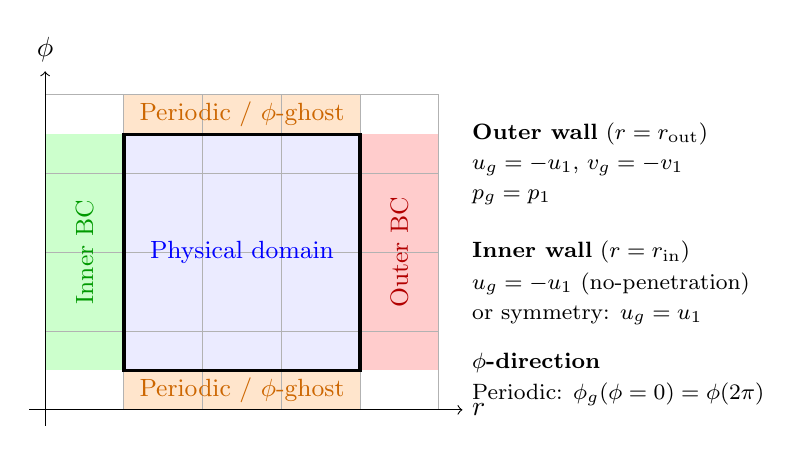
\begin{tikzpicture}[scale=1.0]
    % Physical: annular sector (displayed as rectangle r-phi)
    \fill[blue!8]  (1,0.5) rectangle (4,3.5);
    % Ghost: inner radius
    \fill[green!20] (0,0.5) rectangle (1,3.5);
    % Ghost: outer radius
    \fill[red!20]  (4,0.5) rectangle (5,3.5);
    % Ghost/periodic: phi min
    \fill[orange!20] (1,0) rectangle (4,0.5);
    % Ghost/periodic: phi max
    \fill[orange!20] (1,3.5) rectangle (4,4);

    % Grid
    \draw[gray!60,thin] (0,0) grid (5,4);
    \draw[black,very thick] (1,0.5) rectangle (4,3.5);

    % Axes
    \draw[->] (-0.2,0) -- (5.3,0) node[right]{$r$};
    \draw[->] (0,-0.2) -- (0,4.3) node[above]{$\phi$};

    % Labels
    \node[blue, font=\small] at (2.5,2)   {Physical domain};
    \node[green!60!black, font=\small, rotate=90] at (0.5,2) {Inner BC};
    \node[red!70!black, font=\small, rotate=90]   at (4.5,2) {Outer BC};
    \node[orange!80!black, font=\small] at (2.5,0.25) {Periodic / $\phi$-ghost};
    \node[orange!80!black, font=\small] at (2.5,3.75) {Periodic / $\phi$-ghost};

    % Annotations
    \node[font=\footnotesize, right] at (5.3,3.5) {\textbf{Outer wall} ($r=r_\text{out}$)};
    \node[font=\footnotesize, right] at (5.3,3.1) {$u_g=-u_1$, $v_g=-v_1$};
    \node[font=\footnotesize, right] at (5.3,2.7) {$p_g=p_1$};

    \node[font=\footnotesize, right] at (5.3,2.0) {\textbf{Inner wall} ($r=r_\text{in}$)};
    \node[font=\footnotesize, right] at (5.3,1.6) {$u_g=-u_1$ (no-penetration)};
    \node[font=\footnotesize, right] at (5.3,1.2) {or symmetry: $u_g=u_1$};

    \node[font=\footnotesize, right] at (5.3,0.6) {\textbf{$\phi$-direction}};
    \node[font=\footnotesize, right] at (5.3,0.2) {Periodic: $\phi_g(\phi=0)=\phi(2\pi)$};
\end{tikzpicture}
\caption{Ghost cell layout for the $(r,\phi)$ domain shown as a flattened rectangle. Green: inner radial BC; red: outer radial BC; orange: azimuthal boundary (periodic for a full annulus).}
\label{fig:cyl_uv_ghost}
\end{figure}

\begin{center}
\begin{tabular}{llll}
\toprule
Boundary & Condition & Variable & Ghost value \\
\midrule
Inner wall ($r=r_\text{in}$)  & No-slip: $u=0$, $v=0$  & $u$ & $u_g = -u_1$ \\
                               &                        & $v$ & $v_g = -v_1$ \\
                               & $\partial p/\partial r=0$ & $p$ & $p_g = p_1$ \\
\midrule
Outer wall ($r=r_\text{out}$) & No-slip: $u=0$, $v=0$  & $u$ & $u_g = -u_1$ \\
                               &                        & $v$ & $v_g = -v_1$ \\
                               & $\partial p/\partial r=0$ & $p$ & $p_g = p_1$ \\
\midrule
Azimuthal ($\phi$, full annulus) & Periodic & any $\phi_f$ & $\phi_g(\phi=0) = \phi_f(\phi=2\pi)$ \\
\midrule
Symmetry axis ($r=0$, if present) & $u=0$, $\partial v/\partial r=0$ & $u$ & $u_g=-u_1$ \\
                                   &                                   & $v$ & $v_g = v_1$ \\
\bottomrule
\end{tabular}
\end{center}

\subsubsection{Summary of Correction Equations (all three cases)}

For quick reference, the velocity correction equations for all three coordinate systems are:

\begin{center}
\renewcommand{\arraystretch}{2.0}
\begin{tabular}{lll}
\toprule
System & $u$-correction & $v$ (or $w$)-correction \\
\midrule
Cartesian $(x,y)$
  & $u^{n+1}_{i+\frac{1}{2},j} = u^*_{i+\frac{1}{2},j} - \dfrac{\Delta t}{\rho}\dfrac{p'_{i+1,j}-p'_{i,j}}{\Delta x}$
  & $v^{n+1}_{i,j+\frac{1}{2}} = v^*_{i,j+\frac{1}{2}} - \dfrac{\Delta t}{\rho}\dfrac{p'_{i,j+1}-p'_{i,j}}{\Delta y}$ \\[6pt]
Cylindrical $(r,z)$
  & $u^{n+1}_{i+\frac{1}{2},j} = u^*_{i+\frac{1}{2},j} - \dfrac{\Delta t}{\rho}\dfrac{p'_{i+1,j}-p'_{i,j}}{\Delta r}$
  & $w^{n+1}_{i,j+\frac{1}{2}} = w^*_{i,j+\frac{1}{2}} - \dfrac{\Delta t}{\rho}\dfrac{p'_{i,j+1}-p'_{i,j}}{\Delta z}$ \\[6pt]
Cylindrical $(r,\phi)$
  & $u^{n+1}_{i+\frac{1}{2},j} = u^*_{i+\frac{1}{2},j} - \dfrac{\Delta t}{\rho}\dfrac{p'_{i+1,j}-p'_{i,j}}{\Delta r}$
  & $v^{n+1}_{i,j+\frac{1}{2}} = v^*_{i,j+\frac{1}{2}} - \dfrac{\Delta t}{\rho}\dfrac{2}{r_i}\dfrac{p'_{i,j+1}-p'_{i,j}}{\phi_{j+1}-\phi_{j-1}}$ \\
\bottomrule
\end{tabular}
\end{center}

The extra $1/r_i$ factor in the $(r,\phi)$ case reflects the metric coefficient of the azimuthal gradient.


\end{document}
